% Options for packages loaded elsewhere
\PassOptionsToPackage{unicode}{hyperref}
\PassOptionsToPackage{hyphens}{url}
\PassOptionsToPackage{dvipsnames,svgnames,x11names}{xcolor}
%
\documentclass[
  letterpaper,
  DIV=11,
  numbers=noendperiod]{scrreprt}

\usepackage{amsmath,amssymb}
\usepackage{iftex}
\ifPDFTeX
  \usepackage[T1]{fontenc}
  \usepackage[utf8]{inputenc}
  \usepackage{textcomp} % provide euro and other symbols
\else % if luatex or xetex
  \usepackage{unicode-math}
  \defaultfontfeatures{Scale=MatchLowercase}
  \defaultfontfeatures[\rmfamily]{Ligatures=TeX,Scale=1}
\fi
\usepackage{lmodern}
\ifPDFTeX\else  
    % xetex/luatex font selection
\fi
% Use upquote if available, for straight quotes in verbatim environments
\IfFileExists{upquote.sty}{\usepackage{upquote}}{}
\IfFileExists{microtype.sty}{% use microtype if available
  \usepackage[]{microtype}
  \UseMicrotypeSet[protrusion]{basicmath} % disable protrusion for tt fonts
}{}
\makeatletter
\@ifundefined{KOMAClassName}{% if non-KOMA class
  \IfFileExists{parskip.sty}{%
    \usepackage{parskip}
  }{% else
    \setlength{\parindent}{0pt}
    \setlength{\parskip}{6pt plus 2pt minus 1pt}}
}{% if KOMA class
  \KOMAoptions{parskip=half}}
\makeatother
\usepackage{xcolor}
\setlength{\emergencystretch}{3em} % prevent overfull lines
\setcounter{secnumdepth}{5}
% Make \paragraph and \subparagraph free-standing
\makeatletter
\ifx\paragraph\undefined\else
  \let\oldparagraph\paragraph
  \renewcommand{\paragraph}{
    \@ifstar
      \xxxParagraphStar
      \xxxParagraphNoStar
  }
  \newcommand{\xxxParagraphStar}[1]{\oldparagraph*{#1}\mbox{}}
  \newcommand{\xxxParagraphNoStar}[1]{\oldparagraph{#1}\mbox{}}
\fi
\ifx\subparagraph\undefined\else
  \let\oldsubparagraph\subparagraph
  \renewcommand{\subparagraph}{
    \@ifstar
      \xxxSubParagraphStar
      \xxxSubParagraphNoStar
  }
  \newcommand{\xxxSubParagraphStar}[1]{\oldsubparagraph*{#1}\mbox{}}
  \newcommand{\xxxSubParagraphNoStar}[1]{\oldsubparagraph{#1}\mbox{}}
\fi
\makeatother

\usepackage{color}
\usepackage{fancyvrb}
\newcommand{\VerbBar}{|}
\newcommand{\VERB}{\Verb[commandchars=\\\{\}]}
\DefineVerbatimEnvironment{Highlighting}{Verbatim}{commandchars=\\\{\}}
% Add ',fontsize=\small' for more characters per line
\usepackage{framed}
\definecolor{shadecolor}{RGB}{241,243,245}
\newenvironment{Shaded}{\begin{snugshade}}{\end{snugshade}}
\newcommand{\AlertTok}[1]{\textcolor[rgb]{0.68,0.00,0.00}{#1}}
\newcommand{\AnnotationTok}[1]{\textcolor[rgb]{0.37,0.37,0.37}{#1}}
\newcommand{\AttributeTok}[1]{\textcolor[rgb]{0.40,0.45,0.13}{#1}}
\newcommand{\BaseNTok}[1]{\textcolor[rgb]{0.68,0.00,0.00}{#1}}
\newcommand{\BuiltInTok}[1]{\textcolor[rgb]{0.00,0.23,0.31}{#1}}
\newcommand{\CharTok}[1]{\textcolor[rgb]{0.13,0.47,0.30}{#1}}
\newcommand{\CommentTok}[1]{\textcolor[rgb]{0.37,0.37,0.37}{#1}}
\newcommand{\CommentVarTok}[1]{\textcolor[rgb]{0.37,0.37,0.37}{\textit{#1}}}
\newcommand{\ConstantTok}[1]{\textcolor[rgb]{0.56,0.35,0.01}{#1}}
\newcommand{\ControlFlowTok}[1]{\textcolor[rgb]{0.00,0.23,0.31}{\textbf{#1}}}
\newcommand{\DataTypeTok}[1]{\textcolor[rgb]{0.68,0.00,0.00}{#1}}
\newcommand{\DecValTok}[1]{\textcolor[rgb]{0.68,0.00,0.00}{#1}}
\newcommand{\DocumentationTok}[1]{\textcolor[rgb]{0.37,0.37,0.37}{\textit{#1}}}
\newcommand{\ErrorTok}[1]{\textcolor[rgb]{0.68,0.00,0.00}{#1}}
\newcommand{\ExtensionTok}[1]{\textcolor[rgb]{0.00,0.23,0.31}{#1}}
\newcommand{\FloatTok}[1]{\textcolor[rgb]{0.68,0.00,0.00}{#1}}
\newcommand{\FunctionTok}[1]{\textcolor[rgb]{0.28,0.35,0.67}{#1}}
\newcommand{\ImportTok}[1]{\textcolor[rgb]{0.00,0.46,0.62}{#1}}
\newcommand{\InformationTok}[1]{\textcolor[rgb]{0.37,0.37,0.37}{#1}}
\newcommand{\KeywordTok}[1]{\textcolor[rgb]{0.00,0.23,0.31}{\textbf{#1}}}
\newcommand{\NormalTok}[1]{\textcolor[rgb]{0.00,0.23,0.31}{#1}}
\newcommand{\OperatorTok}[1]{\textcolor[rgb]{0.37,0.37,0.37}{#1}}
\newcommand{\OtherTok}[1]{\textcolor[rgb]{0.00,0.23,0.31}{#1}}
\newcommand{\PreprocessorTok}[1]{\textcolor[rgb]{0.68,0.00,0.00}{#1}}
\newcommand{\RegionMarkerTok}[1]{\textcolor[rgb]{0.00,0.23,0.31}{#1}}
\newcommand{\SpecialCharTok}[1]{\textcolor[rgb]{0.37,0.37,0.37}{#1}}
\newcommand{\SpecialStringTok}[1]{\textcolor[rgb]{0.13,0.47,0.30}{#1}}
\newcommand{\StringTok}[1]{\textcolor[rgb]{0.13,0.47,0.30}{#1}}
\newcommand{\VariableTok}[1]{\textcolor[rgb]{0.07,0.07,0.07}{#1}}
\newcommand{\VerbatimStringTok}[1]{\textcolor[rgb]{0.13,0.47,0.30}{#1}}
\newcommand{\WarningTok}[1]{\textcolor[rgb]{0.37,0.37,0.37}{\textit{#1}}}

\providecommand{\tightlist}{%
  \setlength{\itemsep}{0pt}\setlength{\parskip}{0pt}}\usepackage{longtable,booktabs,array}
\usepackage{calc} % for calculating minipage widths
% Correct order of tables after \paragraph or \subparagraph
\usepackage{etoolbox}
\makeatletter
\patchcmd\longtable{\par}{\if@noskipsec\mbox{}\fi\par}{}{}
\makeatother
% Allow footnotes in longtable head/foot
\IfFileExists{footnotehyper.sty}{\usepackage{footnotehyper}}{\usepackage{footnote}}
\makesavenoteenv{longtable}
\usepackage{graphicx}
\makeatletter
\newsavebox\pandoc@box
\newcommand*\pandocbounded[1]{% scales image to fit in text height/width
  \sbox\pandoc@box{#1}%
  \Gscale@div\@tempa{\textheight}{\dimexpr\ht\pandoc@box+\dp\pandoc@box\relax}%
  \Gscale@div\@tempb{\linewidth}{\wd\pandoc@box}%
  \ifdim\@tempb\p@<\@tempa\p@\let\@tempa\@tempb\fi% select the smaller of both
  \ifdim\@tempa\p@<\p@\scalebox{\@tempa}{\usebox\pandoc@box}%
  \else\usebox{\pandoc@box}%
  \fi%
}
% Set default figure placement to htbp
\def\fps@figure{htbp}
\makeatother

\KOMAoption{captions}{tableheading}
\makeatletter
\@ifpackageloaded{tcolorbox}{}{\usepackage[skins,breakable]{tcolorbox}}
\@ifpackageloaded{fontawesome5}{}{\usepackage{fontawesome5}}
\definecolor{quarto-callout-color}{HTML}{909090}
\definecolor{quarto-callout-note-color}{HTML}{0758E5}
\definecolor{quarto-callout-important-color}{HTML}{CC1914}
\definecolor{quarto-callout-warning-color}{HTML}{EB9113}
\definecolor{quarto-callout-tip-color}{HTML}{00A047}
\definecolor{quarto-callout-caution-color}{HTML}{FC5300}
\definecolor{quarto-callout-color-frame}{HTML}{acacac}
\definecolor{quarto-callout-note-color-frame}{HTML}{4582ec}
\definecolor{quarto-callout-important-color-frame}{HTML}{d9534f}
\definecolor{quarto-callout-warning-color-frame}{HTML}{f0ad4e}
\definecolor{quarto-callout-tip-color-frame}{HTML}{02b875}
\definecolor{quarto-callout-caution-color-frame}{HTML}{fd7e14}
\makeatother
\makeatletter
\@ifpackageloaded{bookmark}{}{\usepackage{bookmark}}
\makeatother
\makeatletter
\@ifpackageloaded{caption}{}{\usepackage{caption}}
\AtBeginDocument{%
\ifdefined\contentsname
  \renewcommand*\contentsname{Table of contents}
\else
  \newcommand\contentsname{Table of contents}
\fi
\ifdefined\listfigurename
  \renewcommand*\listfigurename{List of Figures}
\else
  \newcommand\listfigurename{List of Figures}
\fi
\ifdefined\listtablename
  \renewcommand*\listtablename{List of Tables}
\else
  \newcommand\listtablename{List of Tables}
\fi
\ifdefined\figurename
  \renewcommand*\figurename{Figure}
\else
  \newcommand\figurename{Figure}
\fi
\ifdefined\tablename
  \renewcommand*\tablename{Table}
\else
  \newcommand\tablename{Table}
\fi
}
\@ifpackageloaded{float}{}{\usepackage{float}}
\floatstyle{ruled}
\@ifundefined{c@chapter}{\newfloat{codelisting}{h}{lop}}{\newfloat{codelisting}{h}{lop}[chapter]}
\floatname{codelisting}{Listing}
\newcommand*\listoflistings{\listof{codelisting}{List of Listings}}
\makeatother
\makeatletter
\makeatother
\makeatletter
\@ifpackageloaded{caption}{}{\usepackage{caption}}
\@ifpackageloaded{subcaption}{}{\usepackage{subcaption}}
\makeatother

\usepackage{bookmark}

\IfFileExists{xurl.sty}{\usepackage{xurl}}{} % add URL line breaks if available
\urlstyle{same} % disable monospaced font for URLs
\hypersetup{
  colorlinks=true,
  linkcolor={blue},
  filecolor={Maroon},
  citecolor={Blue},
  urlcolor={Blue},
  pdfcreator={LaTeX via pandoc}}


\author{}
\date{}

\begin{document}

\renewcommand*\contentsname{Table of contents}
{
\hypersetup{linkcolor=}
\setcounter{tocdepth}{2}
\tableofcontents
}

\bookmarksetup{startatroot}

\chapter*{Welcome to the Complex Disordered Matter
Course!}\label{welcome-to-the-complex-disordered-matter-course}
\addcontentsline{toc}{chapter}{Welcome to the Complex Disordered Matter
Course!}

\markboth{Welcome to the Complex Disordered Matter Course!}{Welcome to
the Complex Disordered Matter Course!}

\pandocbounded{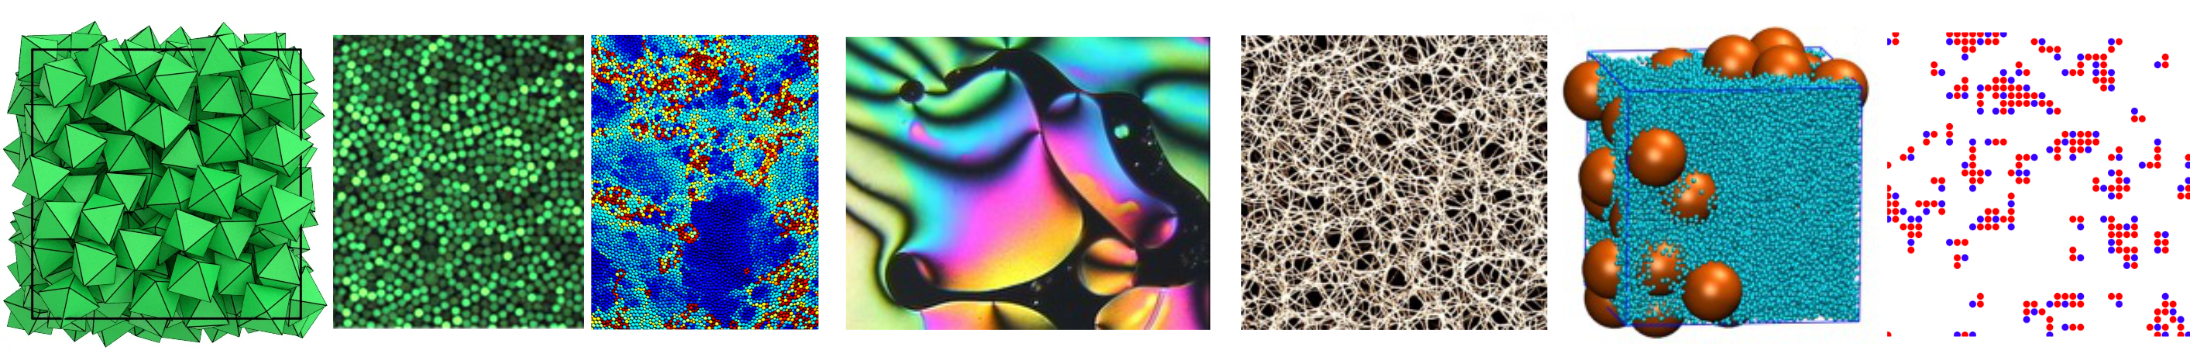
\includegraphics[keepaspectratio]{placeholder_figure_long.png}}\hfill

\section*{Overview}\label{overview}
\addcontentsline{toc}{section}{Overview}

\markright{Overview}

This course introduces your to the theoretical, computational and
experimental aspects of the physics of complex disordered matter.

Complex disordered matter is the study of wide range of systems like
\textbf{polymers}, \textbf{colloids}, \textbf{glasses}, \textbf{gels},
and \textbf{emulsions}, which lack long-range order but exhibit
intricate behaviour. Colloids, suspensions of microscopic particles in a
fluid, are useful for studying disordered structures due to their
observable dynamics. Similarly, polymer systems can form amorphous
solids or glasses when densely packed or cooled, showing solid-like
rigidity despite their disordered structure. These materials often
undergo phase transitions, such as demixing and crystallisation, and
near these transitions, they can display critical phenomena with
extensive fluctuations and correlations.

These various systems are examples of \textbf{soft matter} systems. In
such systems, the interplay between disorder, softness, and phase
behavior leads to rich physical phenomena, particularly near critical
points where even small changes in external conditions can trigger
large-scale reorganisations and universal behaviour. Glasses, for
instance, exhibit slow relaxation and memory effects, while colloidal
systems may crystallize, phase separate, or become jammed depending on
particle interactions and concentration. Understanding such behaviors
involves studying how microscopic interactions and thermal fluctuations
influence macroscopic properties, especially in non-equilibrium
conditions. Through techniques like scattering, microscopy, rheology,
and simulation, one can explore how disordered soft materials respond to
stress, age, or undergo transitions---insights that are vital for
applications in materials design, biotechnology, and beyond.

This course is organized into three interconnected parts, each offering
a distinct perspective on the study of complex disordered matter.

\begin{itemize}
\tightlist
\item
  \textbf{Part 1: Unifying concepts} (Nigel Wilding) introduces the
  theoretical framework for rationalising complex disordered matter
  which is grounded in statistical mechanics and thermodynamics. We
  emphasize the theory of phase transitions, thermal fluctuations,
  critical phenomena, and stochastic dynamics---providing the essential
  theoretical tools needed to describe and predict the behavior of soft
  and disordered systems.\\
\item
  \textbf{Part 2: Complex disordered matter} (Francesco Turci) explores
  the phenomenology of key examples of complex disordered soft matter
  systems, including colloids, polymers, liquid crystals, glasses, gels,
  and active matter. These systems will be analyzed using the
  theoretical concepts introduced in Part 1, highlighting how disorder,
  interactions, and fluctuations shape their macroscopic behavior.\\
\item
  \textbf{Part 3: Experimental techniques} (Adrian Barnes) focuses on
  the methods of microscopy, and scattering via x-rays, neutrons and
  light that are used to study complex disordered matter, offering
  insight into how their properties are measured and understood in
  real-world contexts.
\end{itemize}

In addition to theory and experiment, computer simulation plays a
central role in soft matter research. This course includes a substantial
coursework component consisting of two computational projects. These
exercises will allow you to apply state-of-the-art simulation techniques
to investigate the complex behavior of disordered systems, bridging
theory and observation through hands-on exploration.

\section*{Delivery and format}\label{delivery-and-format}
\addcontentsline{toc}{section}{Delivery and format}

\markright{Delivery and format}

\begin{itemize}
\item
  Detailed e-notes (accessible via Blackboard) can be viewed on a
  variety of devices. Pdf is also available.
\item
  We will give `traditional' lectures (Tuesdays, Wednesdays, Fridays) in
  which we use slides to summarise and explain the lecture content.
  Questions are welcome (within reason\ldots)
\item
  Try to read ahead in the notes, then come to lectures, listen to the
  explanations and then reread the notes.
\item
  Rewriting the notes or slides to express your own thoughts and
  understanding, or annotating a pdf copy can help wire the material
  into your own way of thinking.
\item
  There are problem classes (Thursdays) where you can try problem sheets
  and seek help. Lecturers may go over some problems with the class.
\item
  The navigation bar on the left will allow you to access the lecture
  notes and problem sets.
\end{itemize}

\section*{Intended learning outcomes}\label{intended-learning-outcomes}
\addcontentsline{toc}{section}{Intended learning outcomes}

\markright{Intended learning outcomes}

The course will

\begin{itemize}
\tightlist
\item
  Introduce you to the qualitative features of a range of complex and
  disordered systems and the experimental techniques used to study them.
\item
  Introduce you to a range of model systems and theoretical techniques
  used to elucidate the physics of complex disordered matter.
\item
  Provide you with elementary computational tools to model complex
  disordered systems numerically and predict their properties.
\item
  Allow you to apply your physics background to understand a variety of
  systems of inter-disciplinary relevance.
\item
  Connect with the most recent advances in the research on complex
  disordered matter.
\end{itemize}

\section*{Contact details}\label{contact-details}
\addcontentsline{toc}{section}{Contact details}

\markright{Contact details}

The course will be taught by

\begin{itemize}
\tightlist
\item
  Prof Nigel B. Wilding (unit director): nigel.wilding@bristol.ac.uk
\item
  Dr Francesco Turci: F.Turci@bristol.ac.uk
\item
  Dr Adrian Barnes: a.c.barnes@bristol.ac.uk
\end{itemize}

\section*{Questions and comments}\label{questions-and-comments}
\addcontentsline{toc}{section}{Questions and comments}

\markright{Questions and comments}

If you have any questions about the course, please don't hesitate to
contact the relevant lecturer, either by email (see above) or in a
problems class.

Finally, this is a new course for 2025/26. If you find any errors or
mistakes or something which isn't clear, please let us know by email, or
fill in this anonymous form:

\begin{tcolorbox}[enhanced jigsaw, colframe=quarto-callout-note-color-frame, colback=white, breakable, rightrule=.15mm, arc=.35mm, leftrule=.75mm, bottomrule=.15mm, toprule=.15mm, left=2mm, opacityback=0]

\href{https://forms.office.com/e/YnWKHdiGjv}{Submit an
error/mistake/query}

\end{tcolorbox}

\bookmarksetup{startatroot}

\chapter*{Recommended texts and literature}\label{literature}
\addcontentsline{toc}{chapter}{Recommended texts and literature}

\markboth{Recommended texts and literature}{Recommended texts and
literature}

One motivation for supplying you with detailed notes for this course
course is the absence of a single wholly ideal text book. However, it
should be stressed that while these notes approach (in places) the
detail of a book, the notes are not fully comprehensive and should be
regarded as the `bare bones' of the course, to be fleshed out via your
own reading and supplementary note taking.

\subsection*{Revision on thermodynamics and statistical
mechanics}\label{revision-on-thermodynamics-and-statistical-mechanics}
\addcontentsline{toc}{subsection}{Revision on thermodynamics and
statistical mechanics}

See your year two Thermal Physics notes. Also

\begin{itemize}
\tightlist
\item
  \textbf{\href{https://bris.on.worldcat.org/search/detail/15487191?queryString=F.\%20Mandl&clusterResults=true&stickyFacetsChecked=true&groupVariantRecords=false}{F.
  Mandl: Statistical Physics}}
\end{itemize}

\subsection*{Phase transitions and critical
phenomena}\label{phase-transitions-and-critical-phenomena}
\addcontentsline{toc}{subsection}{Phase transitions and critical
phenomena}

A good book at the right level for the phase transitions and critical
phenomena part of the course is

\begin{itemize}
\tightlist
\item
  \textbf{\href{https://bris.on.worldcat.org/search/detail/24699159?queryString=yeomans\%20statistical&clusterResults=true&stickyFacetsChecked=true&groupVariantRecords=false&newsArticles=off&bookReviews=off}{J.M.
  Yeomans: Statistical Mechanics of Phase Transitions}}
\end{itemize}

A good book covering all aspects of this part of the course including
non-equilibrium systems is

\begin{itemize}
\tightlist
\item
  \textbf{\href{https://bris.on.worldcat.org/search/detail/941821555?queryString=chandler\%20statistical&clusterResults=true&stickyFacetsChecked=true&groupVariantRecords=false&newsArticles=off&bookReviews=off}{D.
  Chandler: Introduction to Modern Statistical Mechanics}}
\end{itemize}

You might also wish to dip into the introductory chapters of the
following more advanced texts

\begin{itemize}
\item
  \textbf{\href{https://bris.on.worldcat.org/search/detail/25914535?queryString=Lectures\%20on\%20Phase\%20Transitions\%20and\%20the\%20Renormalization\%20Group&clusterResults=true&stickyFacetsChecked=true&groupVariantRecords=false&newsArticles=off&bookReviews=off}{N
  Goldenfeld: Lectures on Phase Transitions and the Renormalization
  Group}}
\item
  \textbf{\href{https://bris.on.worldcat.org/search/detail/861559276?queryString=\%20The\%20Theory\%20of\%20Critical\%20Phenomena&clusterResults=true&stickyFacetsChecked=true&groupVariantRecords=false&newsArticles=off&bookReviews=off}{J.J.
  Binney, N.J. Dowrick, A.J.Fisher and M.E.J. Newman: The Theory of
  Critical Phenomena}}
\end{itemize}

\subsection*{Stochastic dynamics}\label{stochastic-dynamics}
\addcontentsline{toc}{subsection}{Stochastic dynamics}

\begin{itemize}
\tightlist
\item
  \textbf{\href{https://bris.on.worldcat.org/search/detail/162131511?queryString=Stochastic\%20Processes\%20in\%20Physics\%20and\%20Chemistry\%20by\%20N.G.\%20van\%20Kampen&clusterResults=true&stickyFacetsChecked=true&groupVariantRecords=false}{N.G.
  van Kampen: Stochastic processess in Physics and Chemistry}}
\end{itemize}

\subsection*{Soft matter and glasses}\label{soft-matter-and-glasses}
\addcontentsline{toc}{subsection}{Soft matter and glasses}

The best overall text for part 2 of the course is:

\begin{itemize}
\tightlist
\item
  \textbf{\href{https://bris.on.worldcat.org/search/detail/48753186?queryString=soft\%20condensed\%20matter&clusterResults=true&stickyFacetsChecked=true&groupVariantRecords=false}{R.A.L
  Jones, Soft Condensed Matter}}.
\end{itemize}

Additionally, the following more specialised texts (which include
information on experimental techniques) might be useful.

\subsubsection*{Colloids}\label{colloids}
\addcontentsline{toc}{subsubsection}{Colloids}

\begin{itemize}
\tightlist
\item
  \textbf{\href{https://bris.on.worldcat.org/search/detail/39129921?queryString=The\%20Colloidal\%20Domain&clusterResults=true&stickyFacetsChecked=true&groupVariantRecords=false&newsArticles=off&bookReviews=off}{D.F.Evans,
  H.Wennerström: The Colloidal Domain - Where Physics, Chemistry,
  Biology, and Technology Meet}}
\item
  \textbf{\href{https://bris.on.worldcat.org/search/detail/27810428?queryString=Introduction\%20to\%20Modern\%20Colloid\%20Science&clusterResults=true&stickyFacetsChecked=true&groupVariantRecords=false&newsArticles=off&bookReviews=off}{R.J.Hunter:
  Introduction to Modern Colloid Science}}
\item
  \textbf{\href{https://bris.on.worldcat.org/search/detail/18869758?queryString=colloidal\%20dispersions&clusterResults=true&stickyFacetsChecked=true&groupVariantRecords=false&newsArticles=off&bookReviews=off}{W.B.Russel,
  D.A.Saville, W.R.Schowalter: Colloidal Dispersions}}
\item
  \textbf{\href{https://bris.on.worldcat.org/search/detail/232632488?queryString=Basic\%20Principles\%20of\%20Colloid\%20Science&clusterResults=true&stickyFacetsChecked=true&groupVariantRecords=false&newsArticles=off&bookReviews=off}{D.H.Everett:
  Basic Principles of Colloid Science}}
\end{itemize}

\subsubsection*{Polymers and
surfactants}\label{polymers-and-surfactants}
\addcontentsline{toc}{subsubsection}{Polymers and surfactants}

\begin{itemize}
\item
  \textbf{\href{https://bris.on.worldcat.org/search/detail/744914764?queryString=introduction\%20to\%20polymers&clusterResults=true&stickyFacetsChecked=true&groupVariantRecords=false&newsArticles=off&bookReviews=off}{R.J.
  Young and P.A. Lovell: Introduction to polymers}}
\item
  \textbf{\href{https://bris.on.worldcat.org/search/detail/32465842?queryString=introduction\%20to\%20polymer\%20physics&clusterResults=true&stickyFacetsChecked=true&groupVariantRecords=false&newsArticles=off&bookReviews=off}{M.
  Doi: Introduction to polymer physics}}
\item
  \textbf{\href{https://bris.on.worldcat.org/search/detail/961357167?queryString=\%20Intermolecular\%20and\%20Surface\%20Forces&clusterResults=true&stickyFacetsChecked=true&groupVariantRecords=false&newsArticles=off&bookReviews=off}{J.Israelachvili,
  Intermolecular and Surface Forces}}
\end{itemize}

\subsubsection*{Glasses}\label{glasses}
\addcontentsline{toc}{subsubsection}{Glasses}

\begin{itemize}
\tightlist
\item
  \textbf{\href{https://bris.on.worldcat.org/search/detail/21975348?queryString=Glasses\%20and\%20the\%20vitreous\%20state&clusterResults=true&stickyFacetsChecked=true&groupVariantRecords=false&newsArticles=off&bookReviews=off}{J.
  Zarzycki; Glasses and the vitreous state}}
\end{itemize}

\part{Unifying concepts}

\chapter{Introduction to phase behaviour and enhanced
fluctuations}\label{introduction-to-phase-behaviour-and-enhanced-fluctuations}

A phase transition can be defined as a macroscopic rearrangment of the
internal constituents of a system in response to a change in the
thermodynamic conditions to which they are subject. A wide variety of
physical systems undergo such transitions. Understanding the properties
of phase transitions is fundamental to the study of soft and complex
matter, as these systems often exhibit rich and subtle transformations
between different states of organization. Whether in colloidal
suspensions, polymer blends, liquid crystals, or biological materials,
phase transitions underpin a wide range of physical behaviours, from
self-assembly and pattern formation to critical phenomena and dynamical
arrest. By analysing how macroscopic phases emerge from microscopic
interactions and external conditions, one gains crucial insight into the
principles that govern structure, stability, and functionality in these
intricate systems. As such, an understanding of phase transitions not
only enriches theoretical understanding but also informs practical
applications across materials science, biophysics, and nanotechnology.
For these reasons we will devote a large proportion of this course to
the study of phase transitions.

Two classic examples of systems displaying phase transitions are the
ferromagnet and fluid systems. For the magnet, a key observable is the
magnetisation defined as the magnetic moment per spin, given by
\(m=M/N\), with \(N\) the number of spins. \(m\) can be positive or
negative, dependent on whether the spins are aligned `up' or `down'. As
the temperature of a ferromagnet is increased, its net magnetisation
\(|m|\) is observed to decrease smoothly, until at a certain temperature
known as the critical temperature, \(T_c\), it vanishes altogether (see
left part of Figure~\ref{fig-isingpd}). We define the magnetisation to
be the \emph{order parameter} of this phase transition.

One can also envisage applying a magnetic field \(H\) to the system
which, depending on its sign (i.e.~whether it is aligned (positive) or
anti-aligned (negative) relative to the magnetisation axis), favours up
or down spin states respectively, as shown schematically in
Figure~\ref{fig-isingpd} (right part). Changing the sign of the magnetic
field \(H\) for \(T<T_c\) leads to a phase transition chacterised by a
discontinuous jump in \(m\). We shall explore this behaviour in more
detail in section 5.

\begin{figure}

\centering{

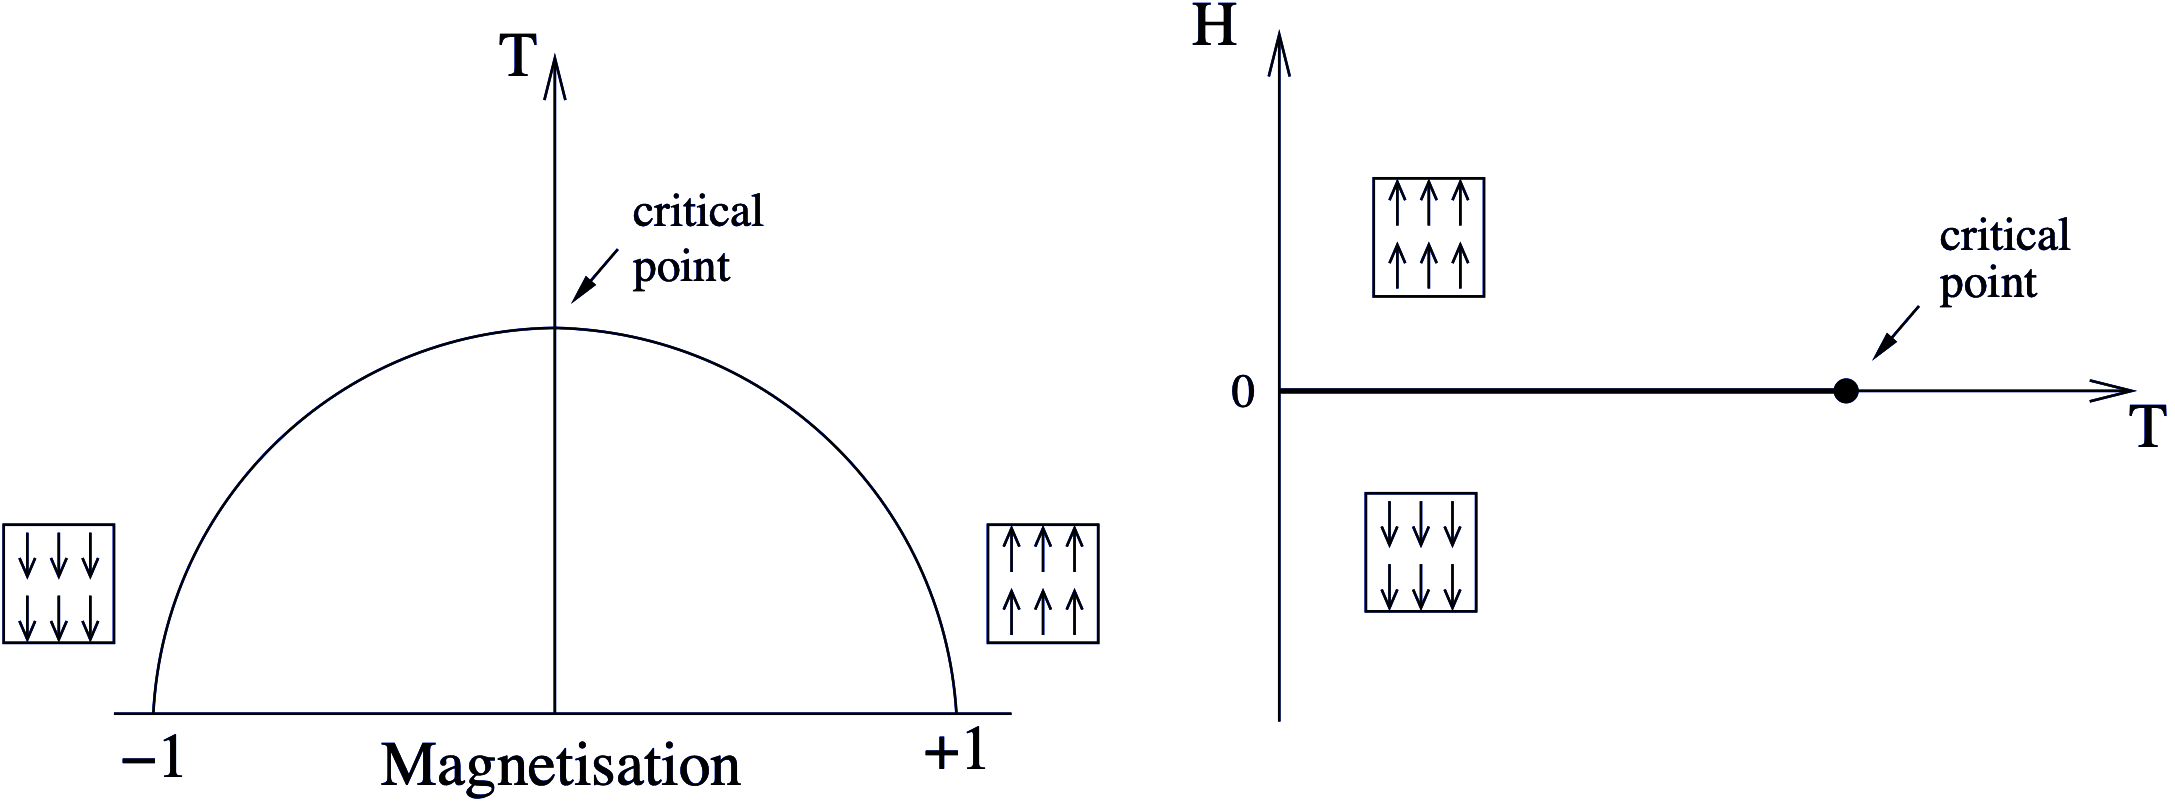
\includegraphics[width=0.8\linewidth,height=\textheight,keepaspectratio]{phase-transitions/Figs/isingpd_color.png}

}

\caption{\label{fig-isingpd}Phase diagram of a simple magnet
(schematic). Left: magnetisation as a function of temperature for zero
applied magnetic field, \(H=0\). Right: Applying a magnetic field that
is aligned or antialigned with the direction of the magnetisation leads
to a phase transition. The \(H=0\) axis at \(T<T_c\) is the coexistence
curve for which positive and negative magnetisations are equally
likely.}

\end{figure}%

Similarly, a change of state from liquid to gas can be induced in a
fluid system (though not in an ideal gas) simply by raising the
temperature. Typically the liquid-vapour transition is abrupt,
reflecting the large number density difference between the states either
side of the transition. However the abruptness of this transition can be
reduced by applying pressure. At one particular pressure and temperature
the discontinuity in the density difference between the two states
vanishes and the two phases coalesce. These conditions of pressure and
temperature serve to locate the critical point for the fluid. We define
the density difference \(\rho_{liq}-\rho_{vap}\) to be the order
parameter for the liquid-gas phase transition. We shall meet order
parameters for other, more complex, systems in section 5,

\begin{figure}

\centering{

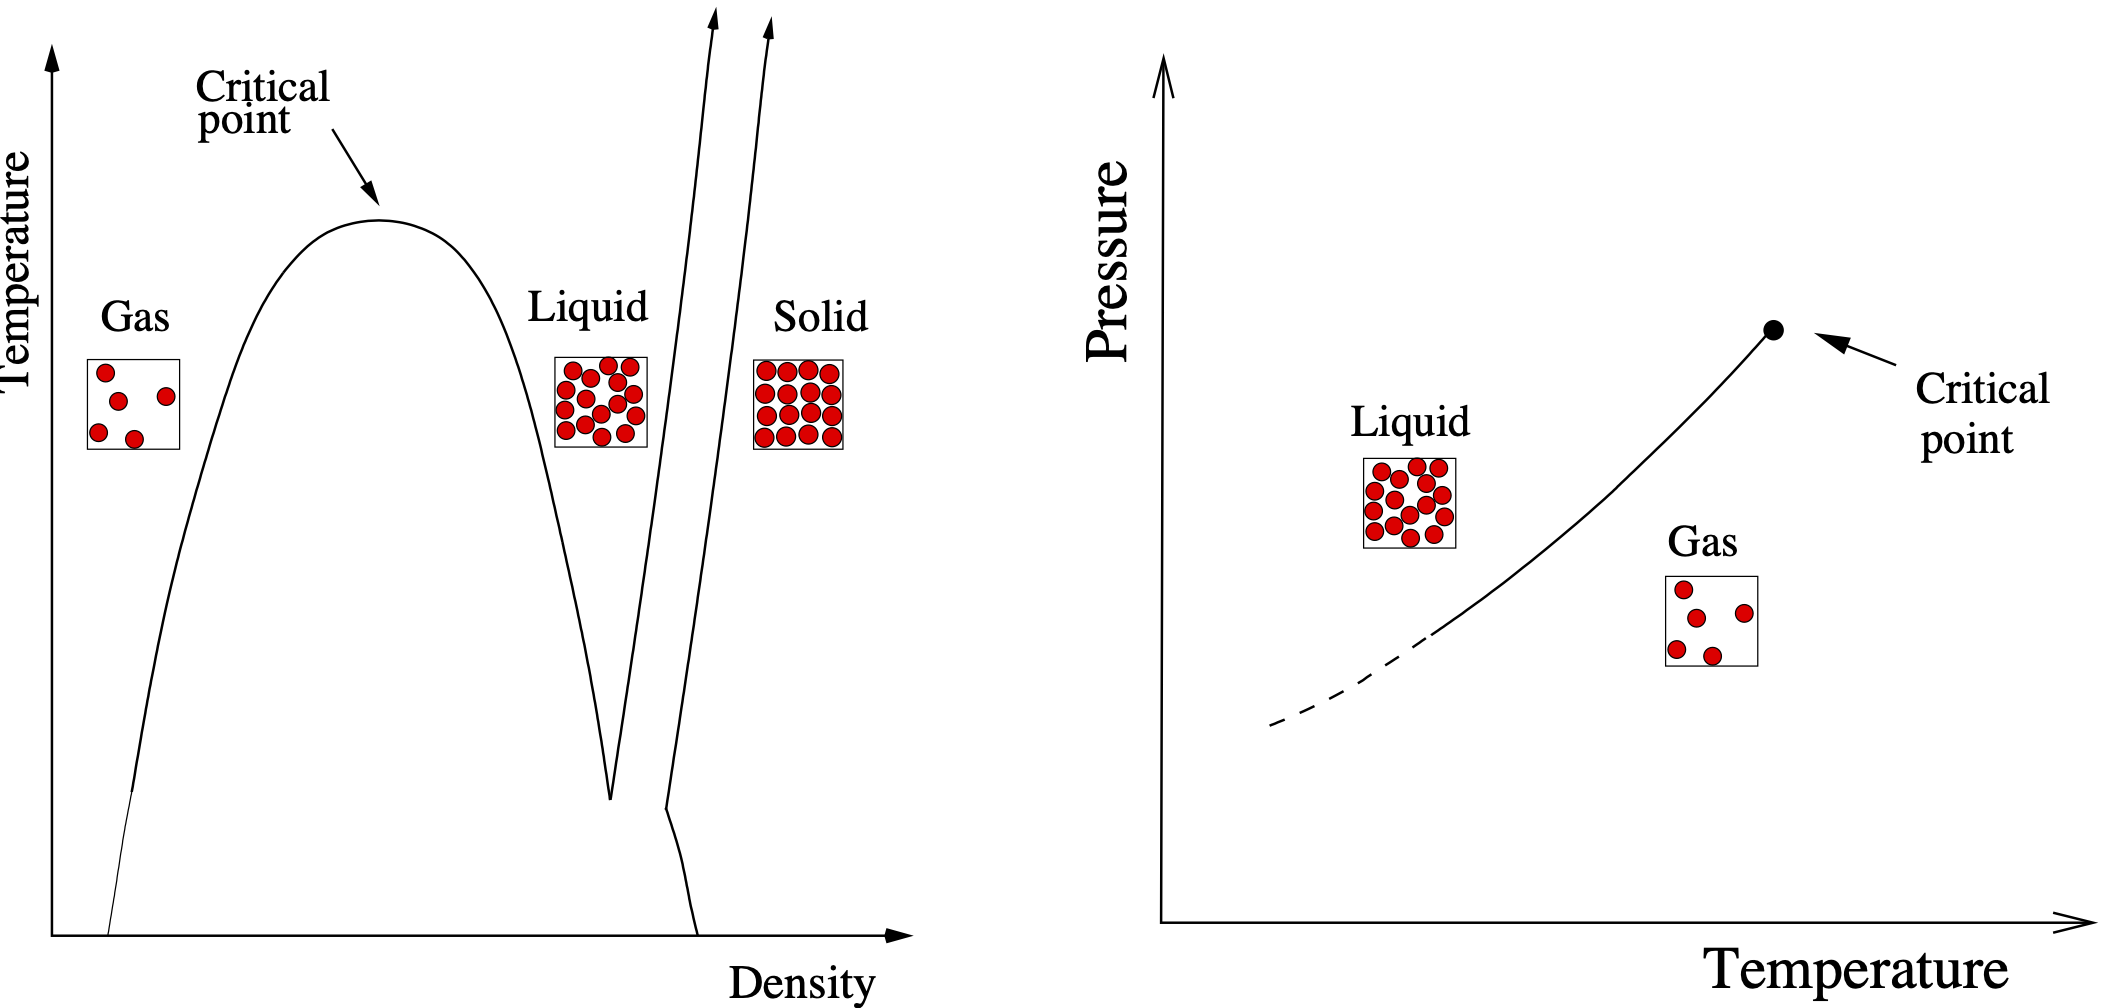
\includegraphics[width=0.8\linewidth,height=\textheight,keepaspectratio]{phase-transitions/Figs/ljpd1.png}

}

\caption{\label{fig-fluidpd}Phase diagram of a simple fluid (schematic)}

\end{figure}%

In the vicinity of a critical point, a system displays a host of
remarkable behaviors known as \emph{critical phenomena}. Chief among
these is the divergence of thermal response functions---such as specific
heat, compressibility, or magnetic susceptibility---which signal an
enhanced sensitivity to external perturbations. These singularities
arise from the emergence of large-scale cooperative interactions among
the system's microscopic constituents, as measured by a diverging
\emph{correlation length} (see Chapter~\ref{sec-background}). One
visually striking manifestation of this is \emph{critical opalescence},
particularly observed in fluids like CO\(_2\). As carbon dioxide nears
its critical temperature and pressure, the distinction between its
liquid and gas phases vanishes, giving rise to huge fluctuations in
density. These fluctuations scatter visible light, rendering the fluid
milky or opalescent. This scattering effect directly reflects the
long-range correlations developing within the fluid. The movie below
illustrates the effect as the critical temperature of CO\(_2\) is
approached from above. Note the appearence of a liquid-vapour interface
(meniscus) as the system enters the two-phase region.

\url{Movies/critical_point_1.mp4}

The recalcitrant problem posed by the critical region is how best to
incorporate such collective effects within the framework of a rigorous
mathematical theory that affords both physical insight and quantitative
explanation of the observed phenomena. This matter has been (and still
is!) the subject of intense theoretical activity.

The importance of the critical point stems largely from the fact that
many of the phenomena observed in its vicinity are believed to be common
to a whole range of apparently quite disparate physical systems. Systems
such as liquid mixtures, superconductors, liquid crystals, ferromagnets,
antiferromagnets and molecular crystals may display identical behaviour
near criticality. This observation implies a profound underlying
similarity among physical systems at criticality, regardless of many
aspects of their distinctive microscopic nature. These ideas have found
formal expression in the so-called `universality hypothesis' which,
since its inception in the 1970s, has enjoyed considerable success.

In the next few lectures, principal aspects of the contemporary
theoretical viewpoint of phase transitions and critical phenomena will
be reviewed. Mean field theories of phase transitions will be discussed
and their inadequacies in the critical region will be exposed. The
phenomenology of the critical region will we described including power
laws, critical exponents and their relationship to scaling phenomena.
These will be set within the context of the powerful renormalisation
group technique. The notion of universality as a phenomenological
hypothesis will be introduced and its implications for real and model
systems will be explored. Finally, the utility of finite-size scaling
methods for computer studies of critical phenomena will be discussed,
culminating in the introduction of a specific technique suitable for
exposing universality in model systems. Thereafter we will consider some
foundational concepts in the dynamics of complex disordered matter. We
shall look at the processes by which one phase transform into another
and introduce differential equations that allow us to deal with the
inherent stochasticity of thermal systems. The wider applicability of
these unifying concepts to complex disordered systems such as colloids,
polymers, liquid crystals and glasses will be covered in part 2 of the
course.

\chapter{Key concepts for phase transitions}\label{sec-background}

\section{Observables and expectation
values}\label{observables-and-expectation-values}

In seeking to describe phase transition and critical phenomena, it is
useful to have a quantitative measure of the difference between the
phases: this is the role of the \emph{order parameter}, \(Q\). In the
case of the fluid, the order parameter is taken as the difference
between the densities of the liquid and vapour phases. In the
ferromagnet it is taken as the magnetisation. As its name suggest, the
order parameter serves as a measure of the kind of orderliness that sets
in when the temperature is cooled below a critical temperature.

Our first task is to give some feeling for the principles which underlie
the ordering process. Referring back to \textbf{?@sec-canonical}, the
probability \(p_a\) that a physical system at temperature \(T\) will
have a particular microscopic arrangement (alternatively referred to as
a `configuration' or `state'), labelled \(a\), of energy \(E_a\) is

\begin{equation}\phantomsection\label{eq-probs}{
p_a=\frac{1}{Z}e^{-E_a/k_BT}
}\end{equation}

The prefactor \(Z^{-1}\) is the \emph{partition function}: since the
system must always have \emph{some} specific arrangement, the sum of the
probabilities \(p_a\) must be unity, implying that

\begin{equation}\phantomsection\label{eq-partition}{
Z=\sum_ae^{-E_a/k_BT}
}\end{equation} where the sum extends over all possible microscopic
arrangements.

These equations assume that physical system evolves rapidly (on the
timescale of typical observations) amongst all its allowed arrangements,
sampling them with the probabilities~Equation~\ref{eq-probs} the
expectation value of any physical observable \(O\) will thus be given by
averaging \(O\) over all the arrangements \(a\), weighting each
contribution by the appropriate probability:

\begin{equation}\phantomsection\label{eq-observable}{\overline {O}=\frac{1}{Z}\sum_a O_a e^{-E_a/k_BT}
}\end{equation}

Sums like Equation~\ref{eq-observable} are not easily evaluated because
the number of terms grows exponentially in the system size.
Nevertheless, some important insights follow painlessly. Consider the
case where the observable of interest is the order parameter, or more
specifically the magnetisation of a ferromagnet.

\begin{equation}\phantomsection\label{eq-op}{
Q=\frac{1}{Z}\sum_a Q_a e^{-E_a/k_BT}
}\end{equation}

It is clear from Equation~\ref{eq-probs} that at very low temperature
the system will be overwhelmingly likely to be found in its minimum
energy arrangements (ground states). For the ferromagnet, these are the
fully ordered spin arrangements having magnetisation \(+1\), or \(-1\).

Now consider the high temperature limit. The enhanced weight that the
fully ordered arrangement carries in the sum of Equation~\ref{eq-op} by
virtue of its low energy, is now no longer sufficient to offset the fact
that arrangements in which \(Q_a\) has some intermediate value, though
each carry a smaller weight, are vastly greater in number. A little
thought shows that the arrangements which have essentially zero
magnetisation (equal populations of up and down spins) are by far the
most numerous. At high temperature, these disordered arrangements
dominate the sum in Equation~\ref{eq-op} and the order parameter is
zero.

The competition between energy-of-arrangements weighting (or simply
`energy') and the `number of arrangements' weighting (or `entropy') is
then the key principle at work here. The distinctive feature of a system
with a critical point is that, in the course of this competition, the
system is forced to choose amongst a number of macroscopically different
sets of microscopic arrangements.

Finally in this section, we note that the probabilistic (statistical
mechanics) approach to thermal systems outlined above is completely
compatible with classical thermodynamics. Specifically, the bridge
between the two disciplines is provided by the following equation

\begin{equation}\phantomsection\label{eq-free}{
F=-k_BT \ln Z
}\end{equation}

where \(F\) is the ``Helmholtz free energy''. All thermodynamic
observables, for example the order parameter \(Q\), and response
functions such as the specific heat or magnetic susceptibility are
obtainable as appropriate derivatives of the free energy. For instance,
utilizing Equation~\ref{eq-partition}, one can readily verify (try it as
an exercise!) that the average internal energy is given by

\[\overline{E}=-\frac{\partial \ln Z}{\partial \beta},\]

where \(\beta=(k_BT)^{-1}\).

The relationship between other thermodynamic quantities and derivatives
of the free energy are given in fig. Figure~\ref{fig-thermo}

\begin{figure}

\centering{

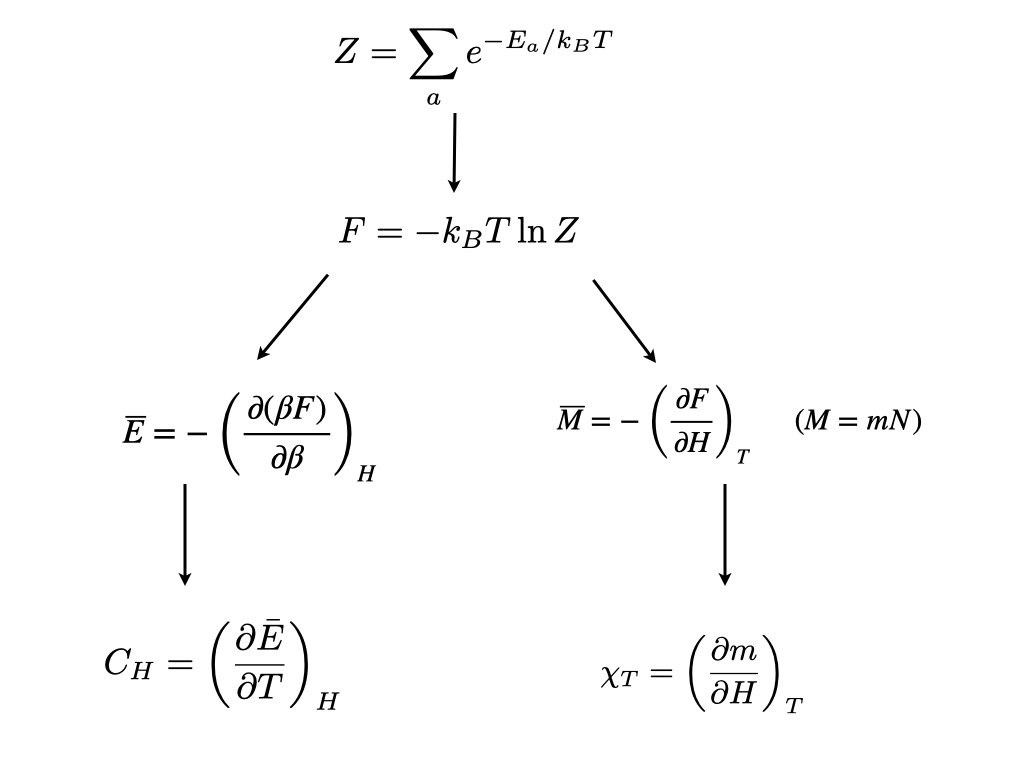
\includegraphics[width=0.8\linewidth,height=\textheight,keepaspectratio]{phase-transitions/Figs/thermo.png}

}

\caption{\label{fig-thermo}Relationships between the partition function
and thermodynamic observables}

\end{figure}%

\section{Correlations}\label{sec-correlations}

\subsection{Spatial correlations}\label{spatial-correlations}

The two-point connected correlation function measures how fluctuations
at two spatial points are statistically related. For a scalar field
\(\phi(\vec{R})\), which could represent eg. the local magnetisation
\(m\) in a magnet at position vector \(\vec{R}\), or the local particle
number density \(\rho\) in a fluid, it is defined as:

\[
C(r) = \langle \phi(\vec{R}) \phi(\vec{R} + \vec{r}) \rangle - \langle \phi(\vec{R}) \rangle^2,
\]

where \(\langle \cdot \rangle\) denotes an ensemble or spatial average
over all \(\vec{R}\), and \(r = |\vec{r}|\) is the spatial separation
between the two points.

\(C(r)\) quantifies the spatial extent over which field values are
correlated and in homogeneous and isotropic systems, it depends only on
the separation \(r\).

If \(C(r)\) decays quickly, we say that correlations are short-ranged.
Typically this occurs well away from criticality and takes the form of
exponential decay

\[
  C(r) \sim e^{-r/\xi}
  \] where the correlation length \(\xi\) is the characteristic scale
over which correlations decay.

Near a critical point \(C(r)\) decays more slowly - in a power-law
fashion - and correlations are long-ranged.

\[
  C(r) \sim r^{-(d - 2 + \eta)}
  \] where \(d\) is the spatial dimension and \(\eta\) is a critical
exponent.

In isotropic fluids and particle systems, a closely related and more
directly measurable quantity (particularly in simulations) is the
\textbf{radial distribution function} \(g(r)\), which describes how
particle density varies as a function of distance from a reference
particle. For such systems, the two-point correlation function of the
number density field \(\rho(\vec{r})\) is related to \(g(r)\) as
follows:

\[
g(r) = 1+\frac{C(r)}{\rho^2},
\] where \(\rho\) is the average number density. This relation shows
that \(g(r)\) encodes the same spatial correlations as \(C(r)\), but in
a form that is more natural for discrete particle systems. Note that by
definition \(g(r)\to 1\) in the absence of correlations ie. when
\(C(r)=0\). This is typically the case for \(r\gg\xi\).

Experimentally one doesn't typically have direct access to \(C(r)\), but
rather its Fourier transform known as the \textbf{structure factor}

\[
S(k) = \int d^d r \, e^{-i \vec{k} \cdot \vec{r}} \, C(r),
\] where \(k\) is the scattering wavevector.

In equilibrium:

\begin{itemize}
\item
  For short-range correlations (finite \(\xi\)), \(S(k)\) typically has
  a Lorentzian form: \[
  S(k) \sim \frac{1}{k^2 + \xi^{-2}}.
  \]
\item
  At criticality (where \(\xi \to \infty\)), \(S(k)\) follows a power
  law: \[
  S(k) \sim k^{-2 + \eta}.
  \]
\end{itemize}

This relation enables the extraction of \(\xi\) from experimental or
simulation data, especially via scattering techniques.

\subsection{Temporal correlations}\label{temporal-correlations}

Consider a thermodynamic variable \(x\) with zero mean that fluctuates
over time. Examples include the local magnetization in a magnetic system
or the local density in a fluid. Here, \(x\) represents a deviation from
the average value --- a fluctuation.

We're interested in how such fluctuations are correlated over time when
the system is in thermal equilibrium. For instance, if \(x\) is positive
at some time \(t\), it's more likely to remain positive shortly after.

These temporal correlations are characterized by the two-time
correlation function (also known as an auto-correlation function):

\[
\langle x(\tau) x(\tau + t) \rangle
\]

In equilibrium, the correlation function must be independent of the
starting time \(\tau\). Therefore, we define:

\[
\langle x(\tau) x(\tau + t) \rangle = M_{xx}(t)
\]

That is, \(M_{xx}(t)\) depends only on the time difference \(t\).

We typically expect \(M_{xx}(t)\) to decay exponentially over a
characteristic correlation time \(t_c\):

\[
M_{xx}(t) \sim \exp(-t / t_c)
\]

\begin{figure}

\centering{

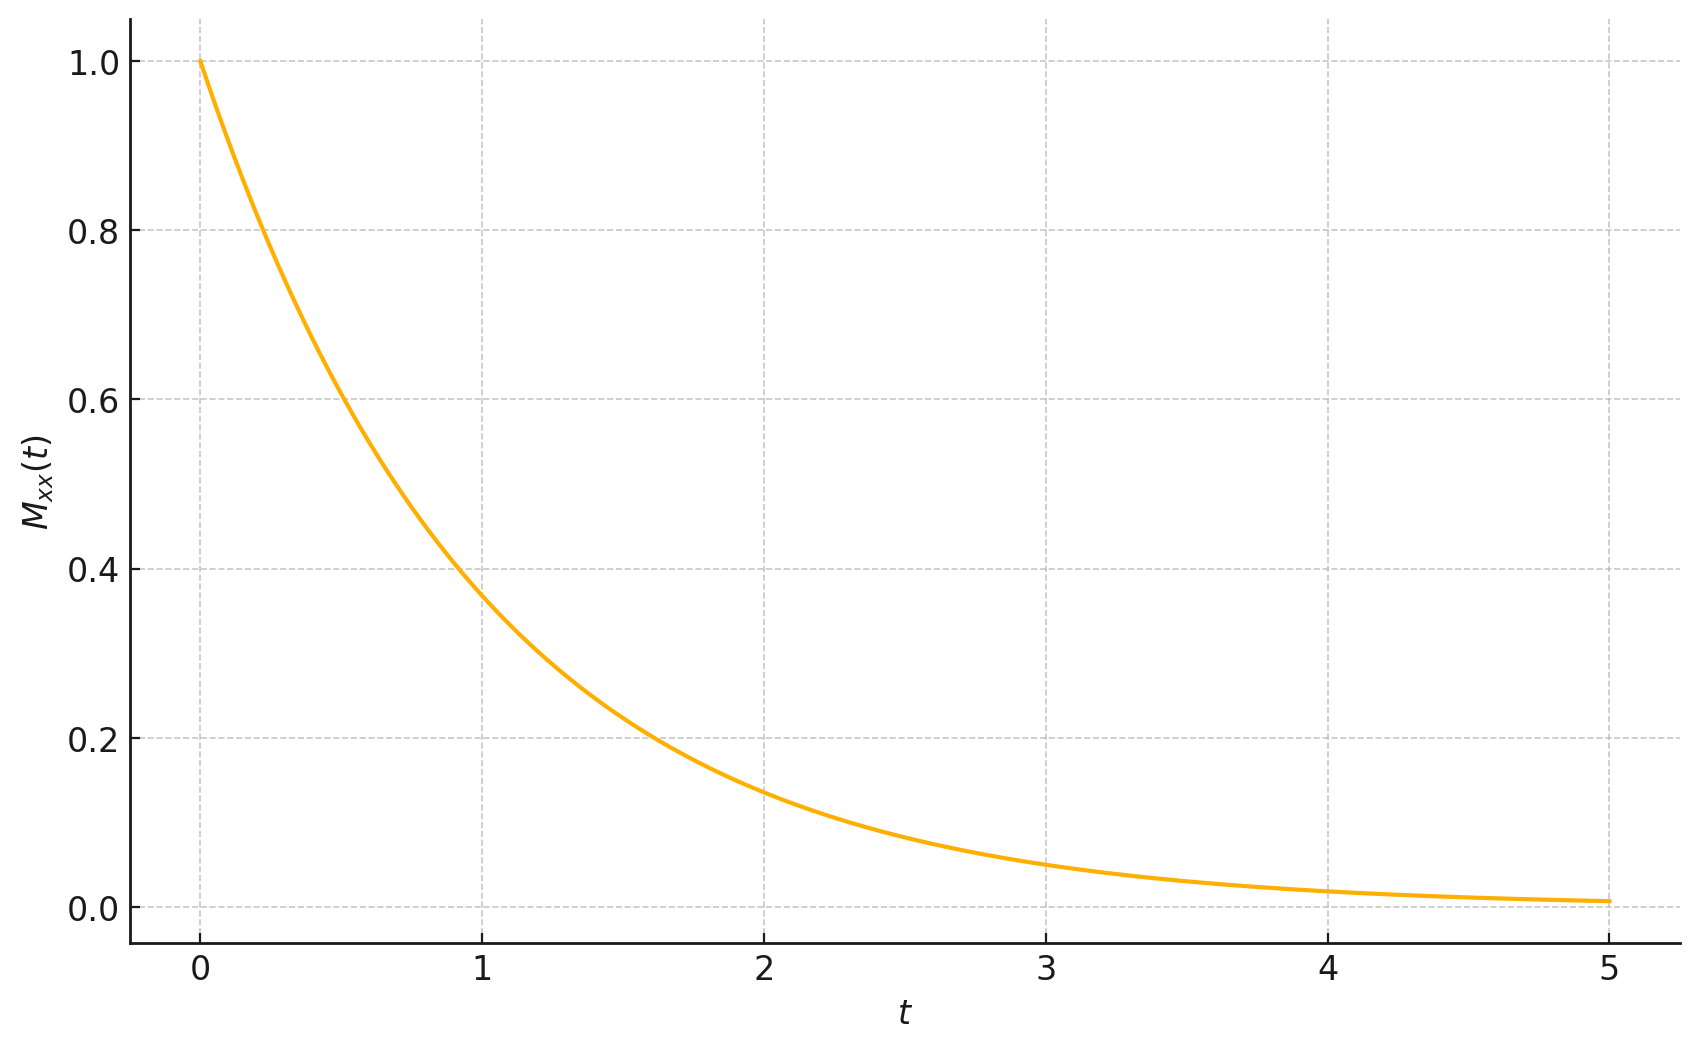
\includegraphics[width=0.6\linewidth,height=\textheight,keepaspectratio]{phase-transitions/Figs/Mxx(t).png}

}

\caption{\label{fig-Mxx}Sketch of \(M_{xx}(t)\) against \(t\)}

\end{figure}%

This exponential decay reflects how the memory of fluctuations fades
with time.

Now consider two different fluctuating variables, \(x\) and \(y\) (e.g.,
local magnetizations at different positions). Their cross-correlation
function is defined as:

\[
\langle x(\tau) y(\tau + t) \rangle = M_{xy}(t)
\]

This defines the elements of a dynamic correlation matrix, of which
\(M_{xx}(t)\) is the diagonal.

\chapter{The approach to criticality}\label{sec:approach}

It is a matter of experimental fact that the approach to criticality in
a given system is characterized by the divergence of various
thermodynamic observables. Let us remain with the archetypal example of
a critical system, the ferromagnet, whose critical temperature will be
denoted as \(T_c\). For temperatures close to \(T_c\), the magnetic
response functions (the magnetic susceptibility \(\chi\) and the
specific heat) are found to be singular functions, diverging as a
\emph{power} of the reduced (dimensionless) temperature \(t \equiv
(T-T_c)/T_c\):-

\begin{equation}\phantomsection\label{eq-chipow}{
\chi \equiv \frac{\partial M}{\partial H}\propto t^{-\gamma} ~~~~ (H=0) 
}\end{equation}

(where \(M=mN\)), \begin{equation}\phantomsection\label{eq-Cv}{
C_H \equiv \frac{\partial E}{\partial T}\propto t^{-\alpha} ~~~~ (H=\textrm{ constant}) 
}\end{equation}

Another key quantity is the correlation length \(\xi\), which measures
the distance over which fluctuations of the magnetic moments are
correlated. This is observed to diverge near the critical point with an
exponent \(\nu\).

\begin{equation}\phantomsection\label{eq-corr}{
\xi \propto t^{-\nu} ~~~~ (T > T_c,\: H=0)
}\end{equation}

Similar power law behaviour is found for the order parameter \(Q\) (in
this case the magnetisation) which vanishes in a singular fashion (it
has infinite gradient) as the critical point is is approached as a
function of temperature:

\begin{equation}\phantomsection\label{eq-mag}{
m \propto t^{\beta} ~~~~ (T < T_c,\: H=0) 
}\end{equation} (here the symbol \(\beta\), is not to be confused with
\(\beta=1/k_BT\)-- this unfortunately is the standard notation.)

Finally, as a function of magnetic field:

\begin{equation}\phantomsection\label{eq-field}{m \propto h^{1/\delta} ~~~~ (T = T_c,\: H>0) .}\end{equation}
with \(h=(H-H_c)/H_c\), the reduced magnetic field.

As examples, the behaviour of the magnetisation and correlation length
are plotted in Figure~\ref{fig-sing} as a function of \(t\).

\begin{figure}

\centering{

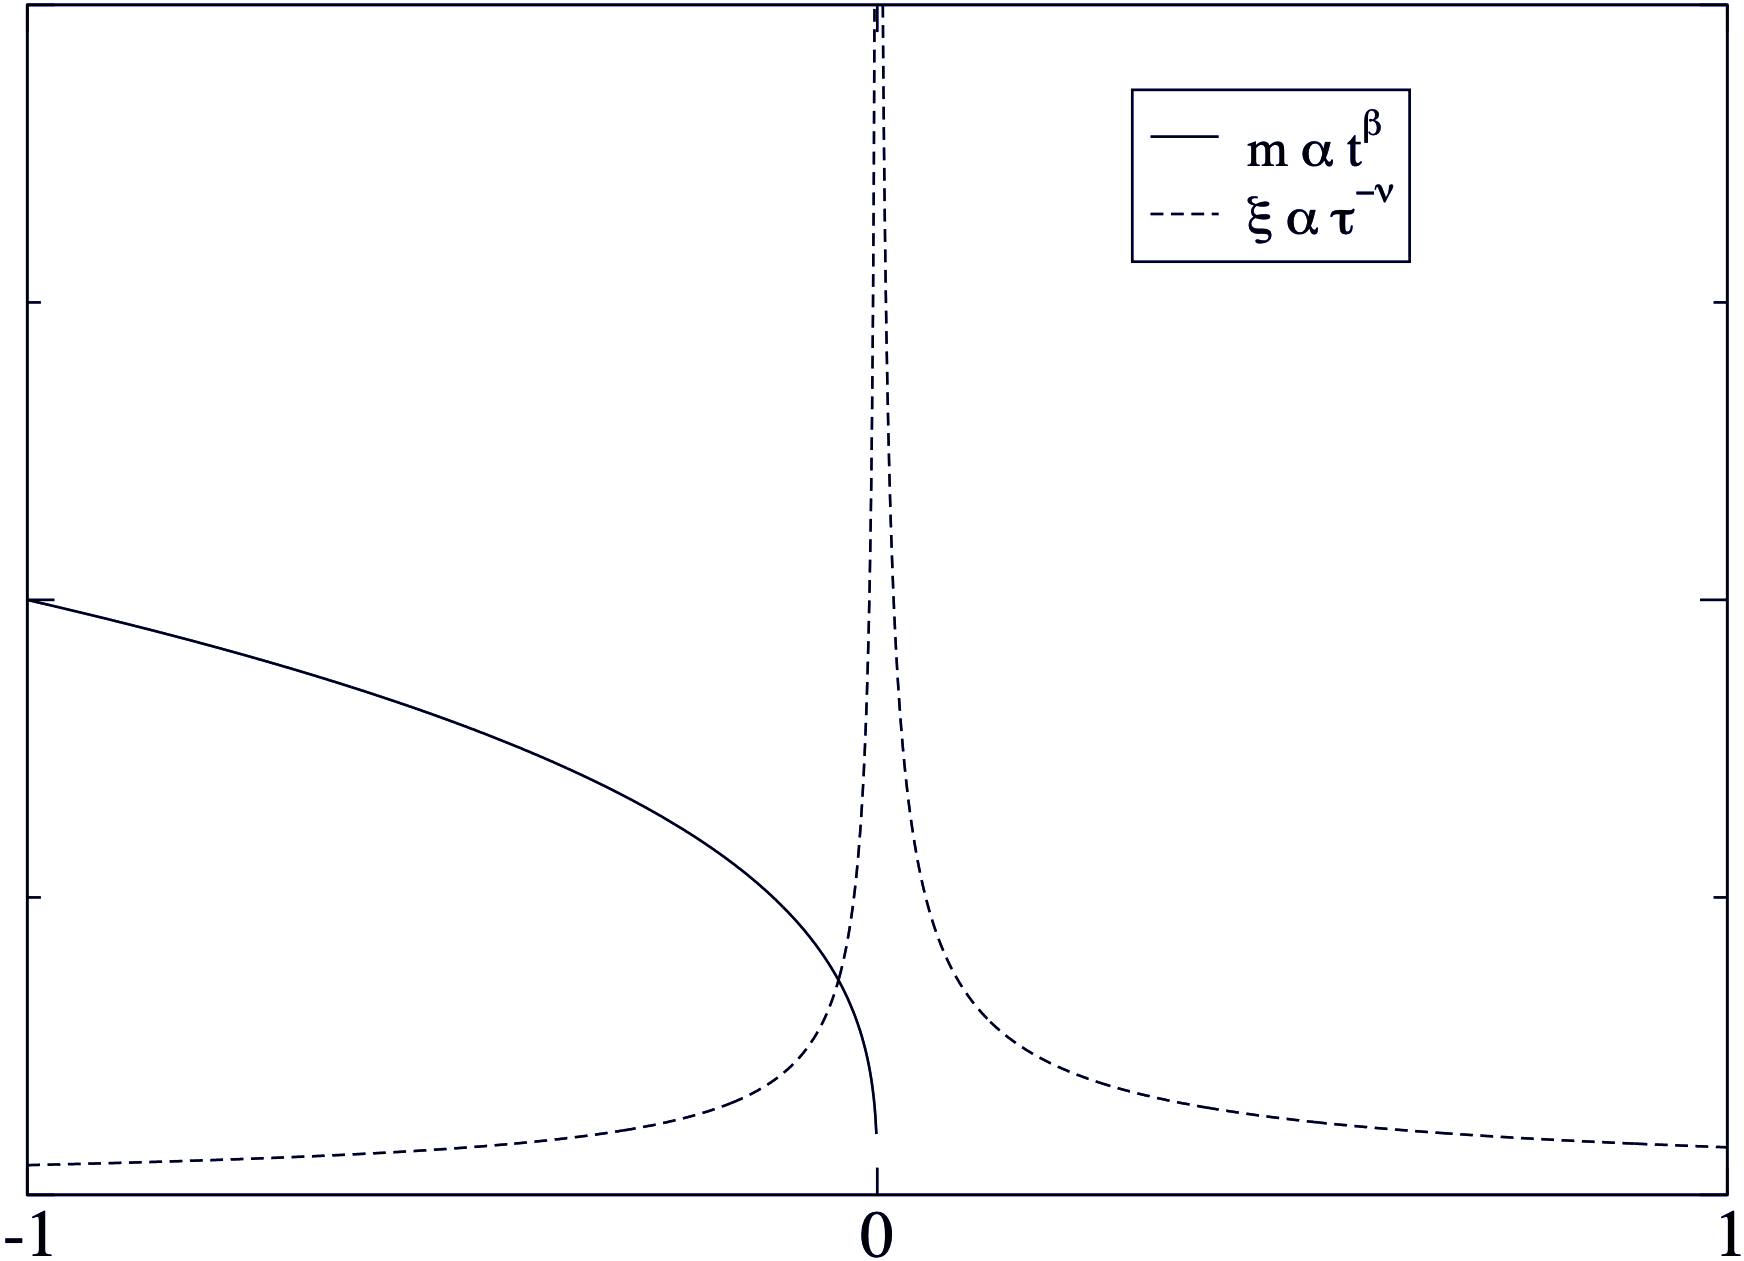
\includegraphics[width=0.5\linewidth,height=\textheight,keepaspectratio]{phase-transitions/Figs/sing_color.png}

}

\caption{\label{fig-sing}Singular behaviour of the correlation length
and order parameter in the vicinity of the critical point as a function
of the reduced temperature \(t\).}

\end{figure}%

The quantities \(\gamma, \alpha, \nu, \beta\) in the above equations are
known as critical exponents. They serve to control the rate at which the
various thermodynamic quantities change on the approach to criticality.

Remarkably, the form of singular behaviour observed at criticality for
the example ferromagnet also occurs in qualitatively quite different
systems such as the fluid. All that is required to obtain the
corresponding power law relationships for the fluid is to substitute the
analogous thermodynamic quantities in to the above equations.
Accordingly the magnetisation order parameter is replaced by the density
difference \(\rho_{liq}-\rho_{gas}\) while the susceptibility is
replaced by the isothermal compressibility and the specific heat
capacity at constant field is replaced by the specific heat capacity at
constant volume. The approach to criticality in a variety of
qualitatively quite different systems can therefore be expressed in
terms of a set of critical exponents describing the power law behaviour
for that system (see the book by Yeomans for examples).

Even more remarkable is the experimental observation that the values of
the critical exponents for a whole range of fluids and magnets (and
indeed many other systems with critical points) are \emph{identical}.
This is the phenomenon of \emph{universality}. It implies a deep
underlying physical similarity between ostensibly disparate critical
systems. The principal aim of theories of critical point phenomena is to
provide a sound theoretical basis for the existence of power law
behaviour, the factors governing the observed values of critical
exponents and the universality phenomenon. Ultimately this basis is
provided by the Renormalisation Group (RG) theory, for which K.G. Wilson
was awarded the Nobel Prize in Physics in 1982.

More about the scientists mentioned in this chapter:

\href{https://en.wikipedia.org/wiki/Kenneth_G._Wilson}{Kenneth Wilson}

\chapter{The Ising model: the prototype model for a phase
transition}\label{sec-Isingmodel}

In order to probe the properties of the critical region, it is common to
appeal to simplified model systems whose behaviour parallels that of
real materials. The sophistication of any particular model depends on
the properties of the system it is supposed to represent. The simplest
model to exhibit critical phenomena is the two-dimensional Ising model
of a ferromagnet. Actual physical realizations of 2-d magnetic systems
do exist in the form of layered ferromagnets such as K\(_2\)CoF\(_4\),
so the 2-d Ising model is of more than just technical relevance.

\section{The 2D Ising model}\label{the-2d-ising-model}

The 2-d spin-\(\frac{1}{2}\) Ising model envisages a regular arrangement
of magnetic moments or `spins' on an infinite plane. Each spin can take
two values, \(+1\) (`up' spins) or \(-1\) (`down' spins) and is assumed
to interact with its nearest neighbours according to the Hamiltonian

\begin{equation}\phantomsection\label{eq-ising}{
{\cal H}_I=-J\sum_{<ij>}s_is_j - H\sum_i s_i
}\end{equation}

where \(J>0\) measures the strength of the coupling between spins and
the sum extends over nearest neighbour spins \(s_i\) and \(s_j\), i.e it
is a sum of the bonds of the lattice. \(H\) is a magnetic field term
which can be positive or negative (although for the time being we will
set it equal to zero). The order parameter is simply the average
magnetisation:

\[m=\frac{1}{N} \langle \sum_i s_i \rangle\:,\] where
\(\langle\cdot\rangle\) means an average over typical configurations
corresponding to the prescribed value of \(J/k_BT\).

The fact that the Ising model displays a phase transition was argued in
Chapter~\ref{sec-background}. Thus at low temperatures for which there
is little thermal disorder, there is a preponderance of aligned spins
and hence a net spontaneous magnetic moment (ie. the system is
ferromagnetic). As the temperature is raised, thermal disorder increases
until at a certain temperature \(T_c\), entropy drives the system
through a continuous phase transition to a disordered spin arrangement
with zero net magnetisation (ie. the system is paramagnetic). These
trends are visible in configurational snapshots from computer
simulations of the 2D Ising model (see Figure~\ref{fig-snapshots}).
Although each spin interacts only with its nearest neighbours, the phase
transition occurs due to cooperative effects among a large number of
spins.

\begin{figure}

\begin{minipage}{0.33\linewidth}

\centering{

\pandocbounded{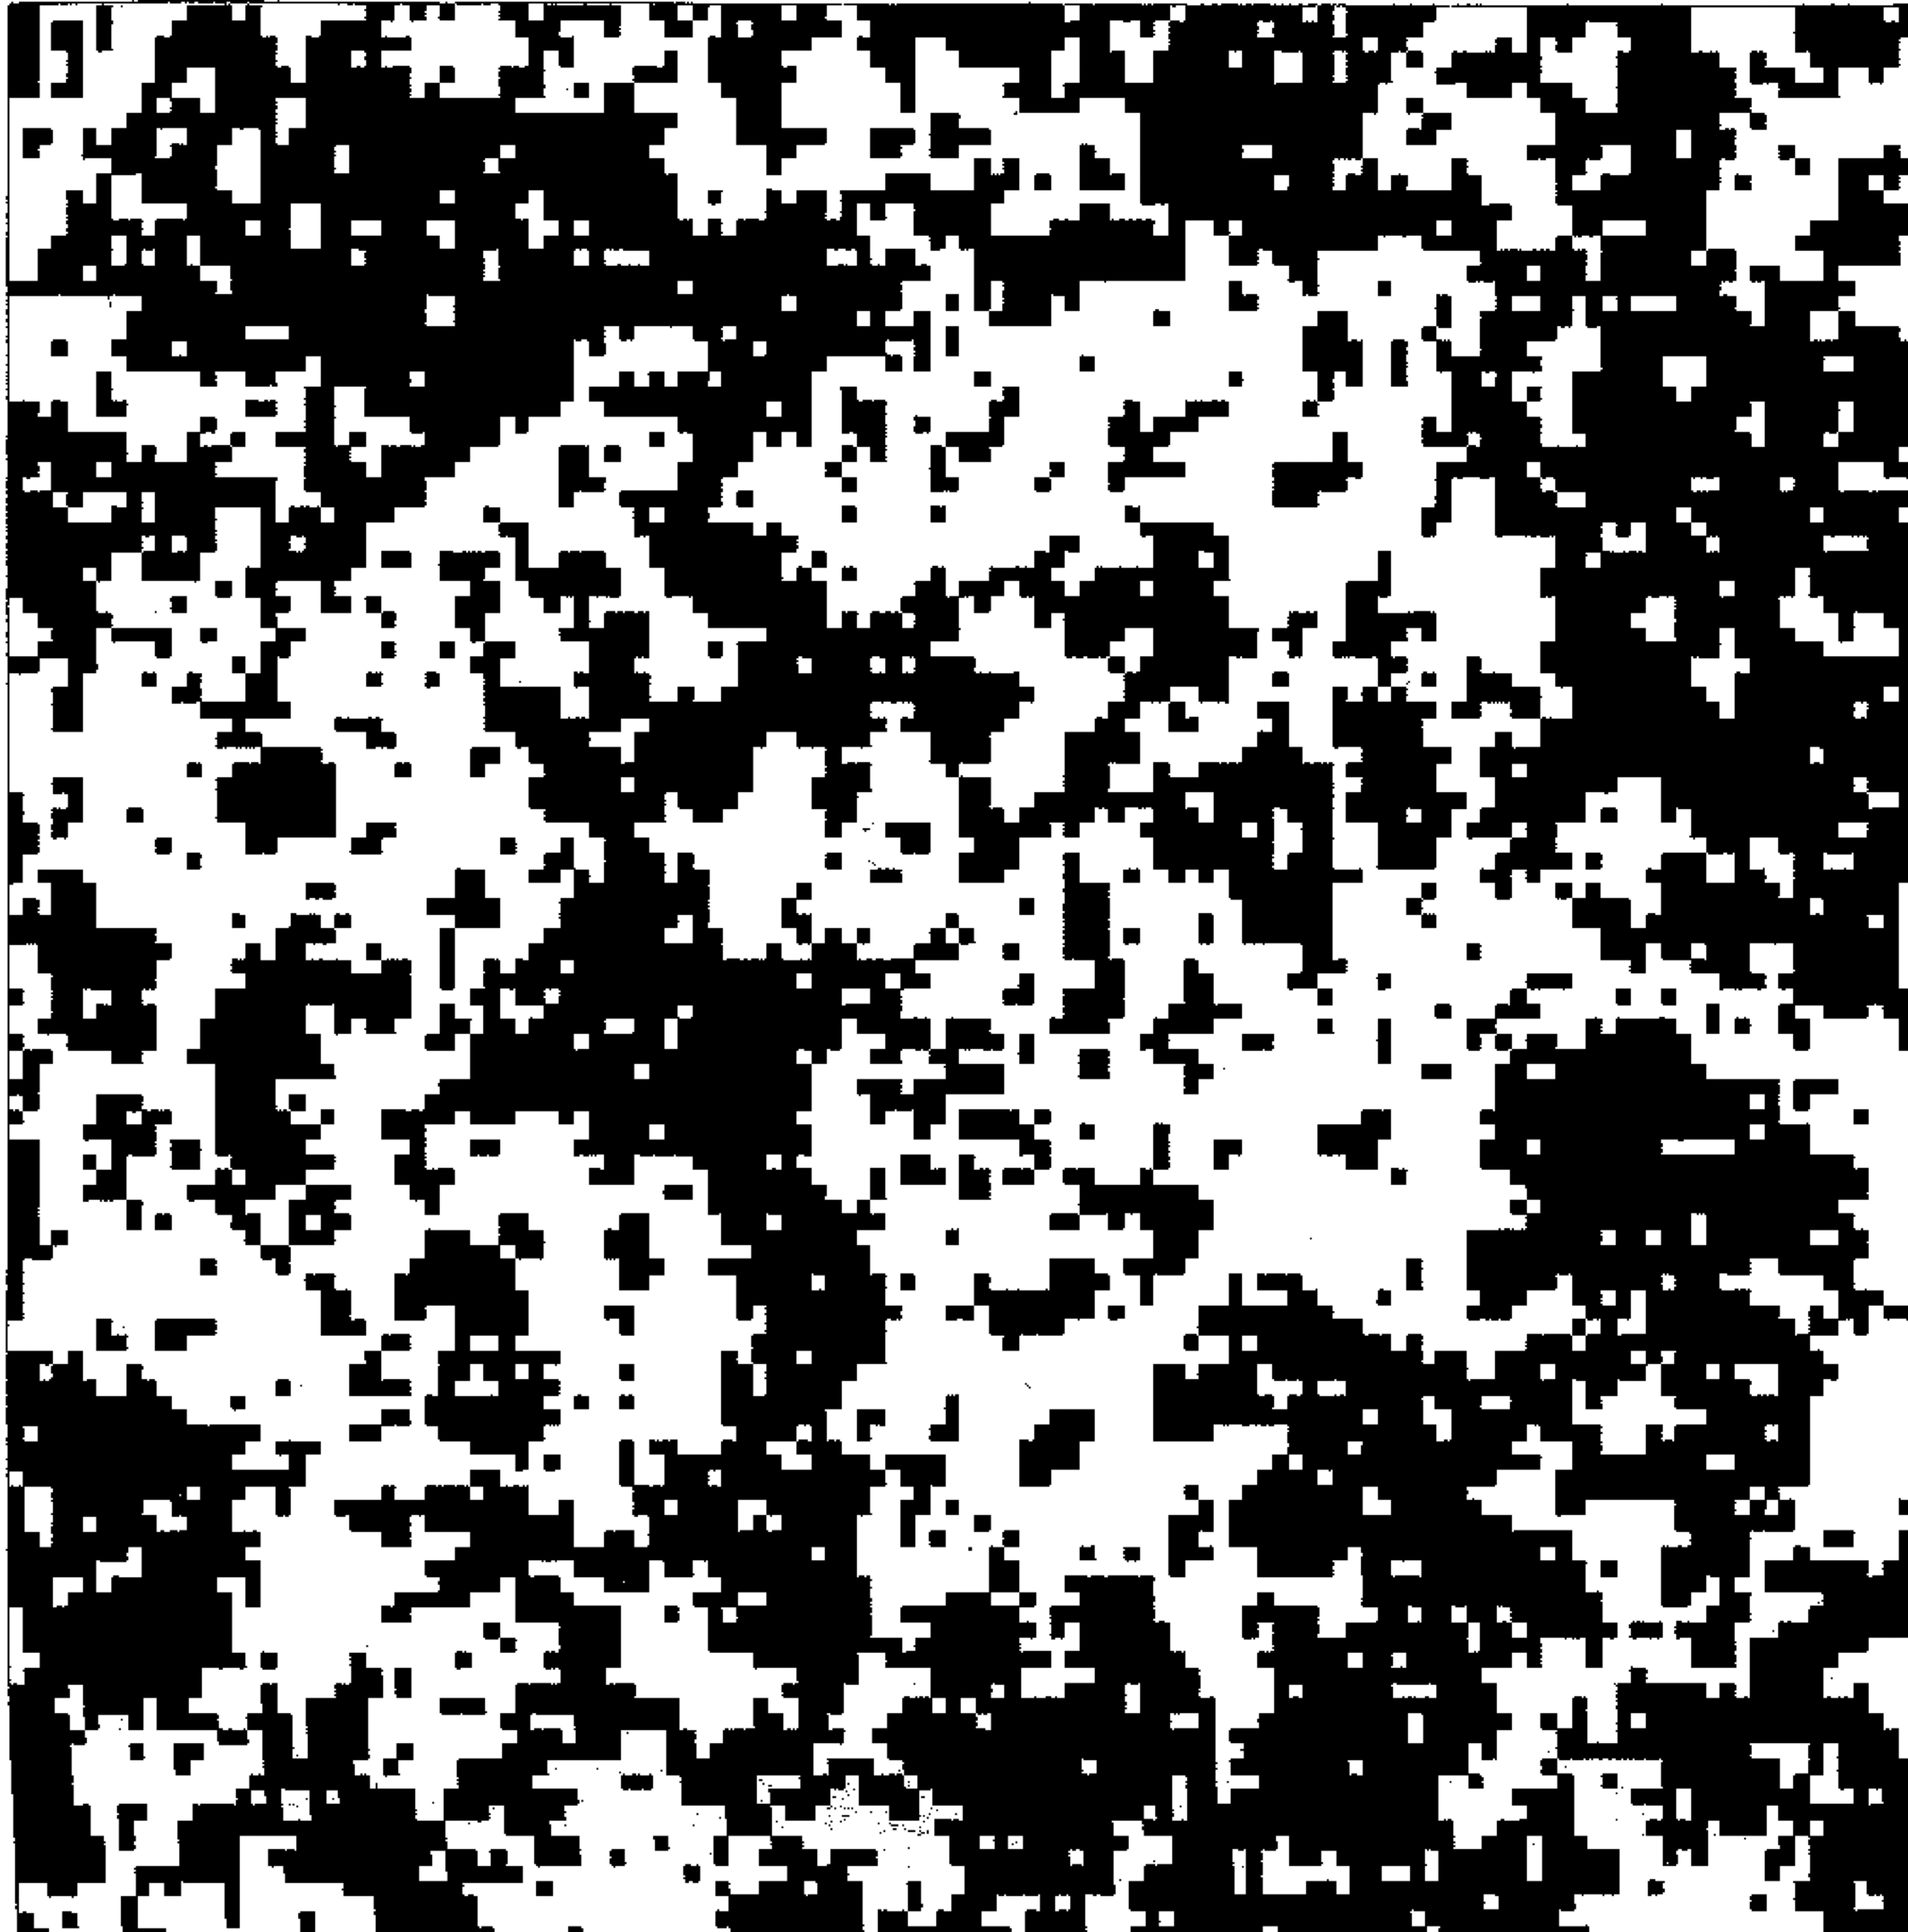
\includegraphics[keepaspectratio]{phase-transitions/Figs/supercrit.png}}

}

\subcaption{\label{fig-ssa}\(T=1.2T_c\)}

\end{minipage}%
%
\begin{minipage}{0.33\linewidth}

\centering{

\pandocbounded{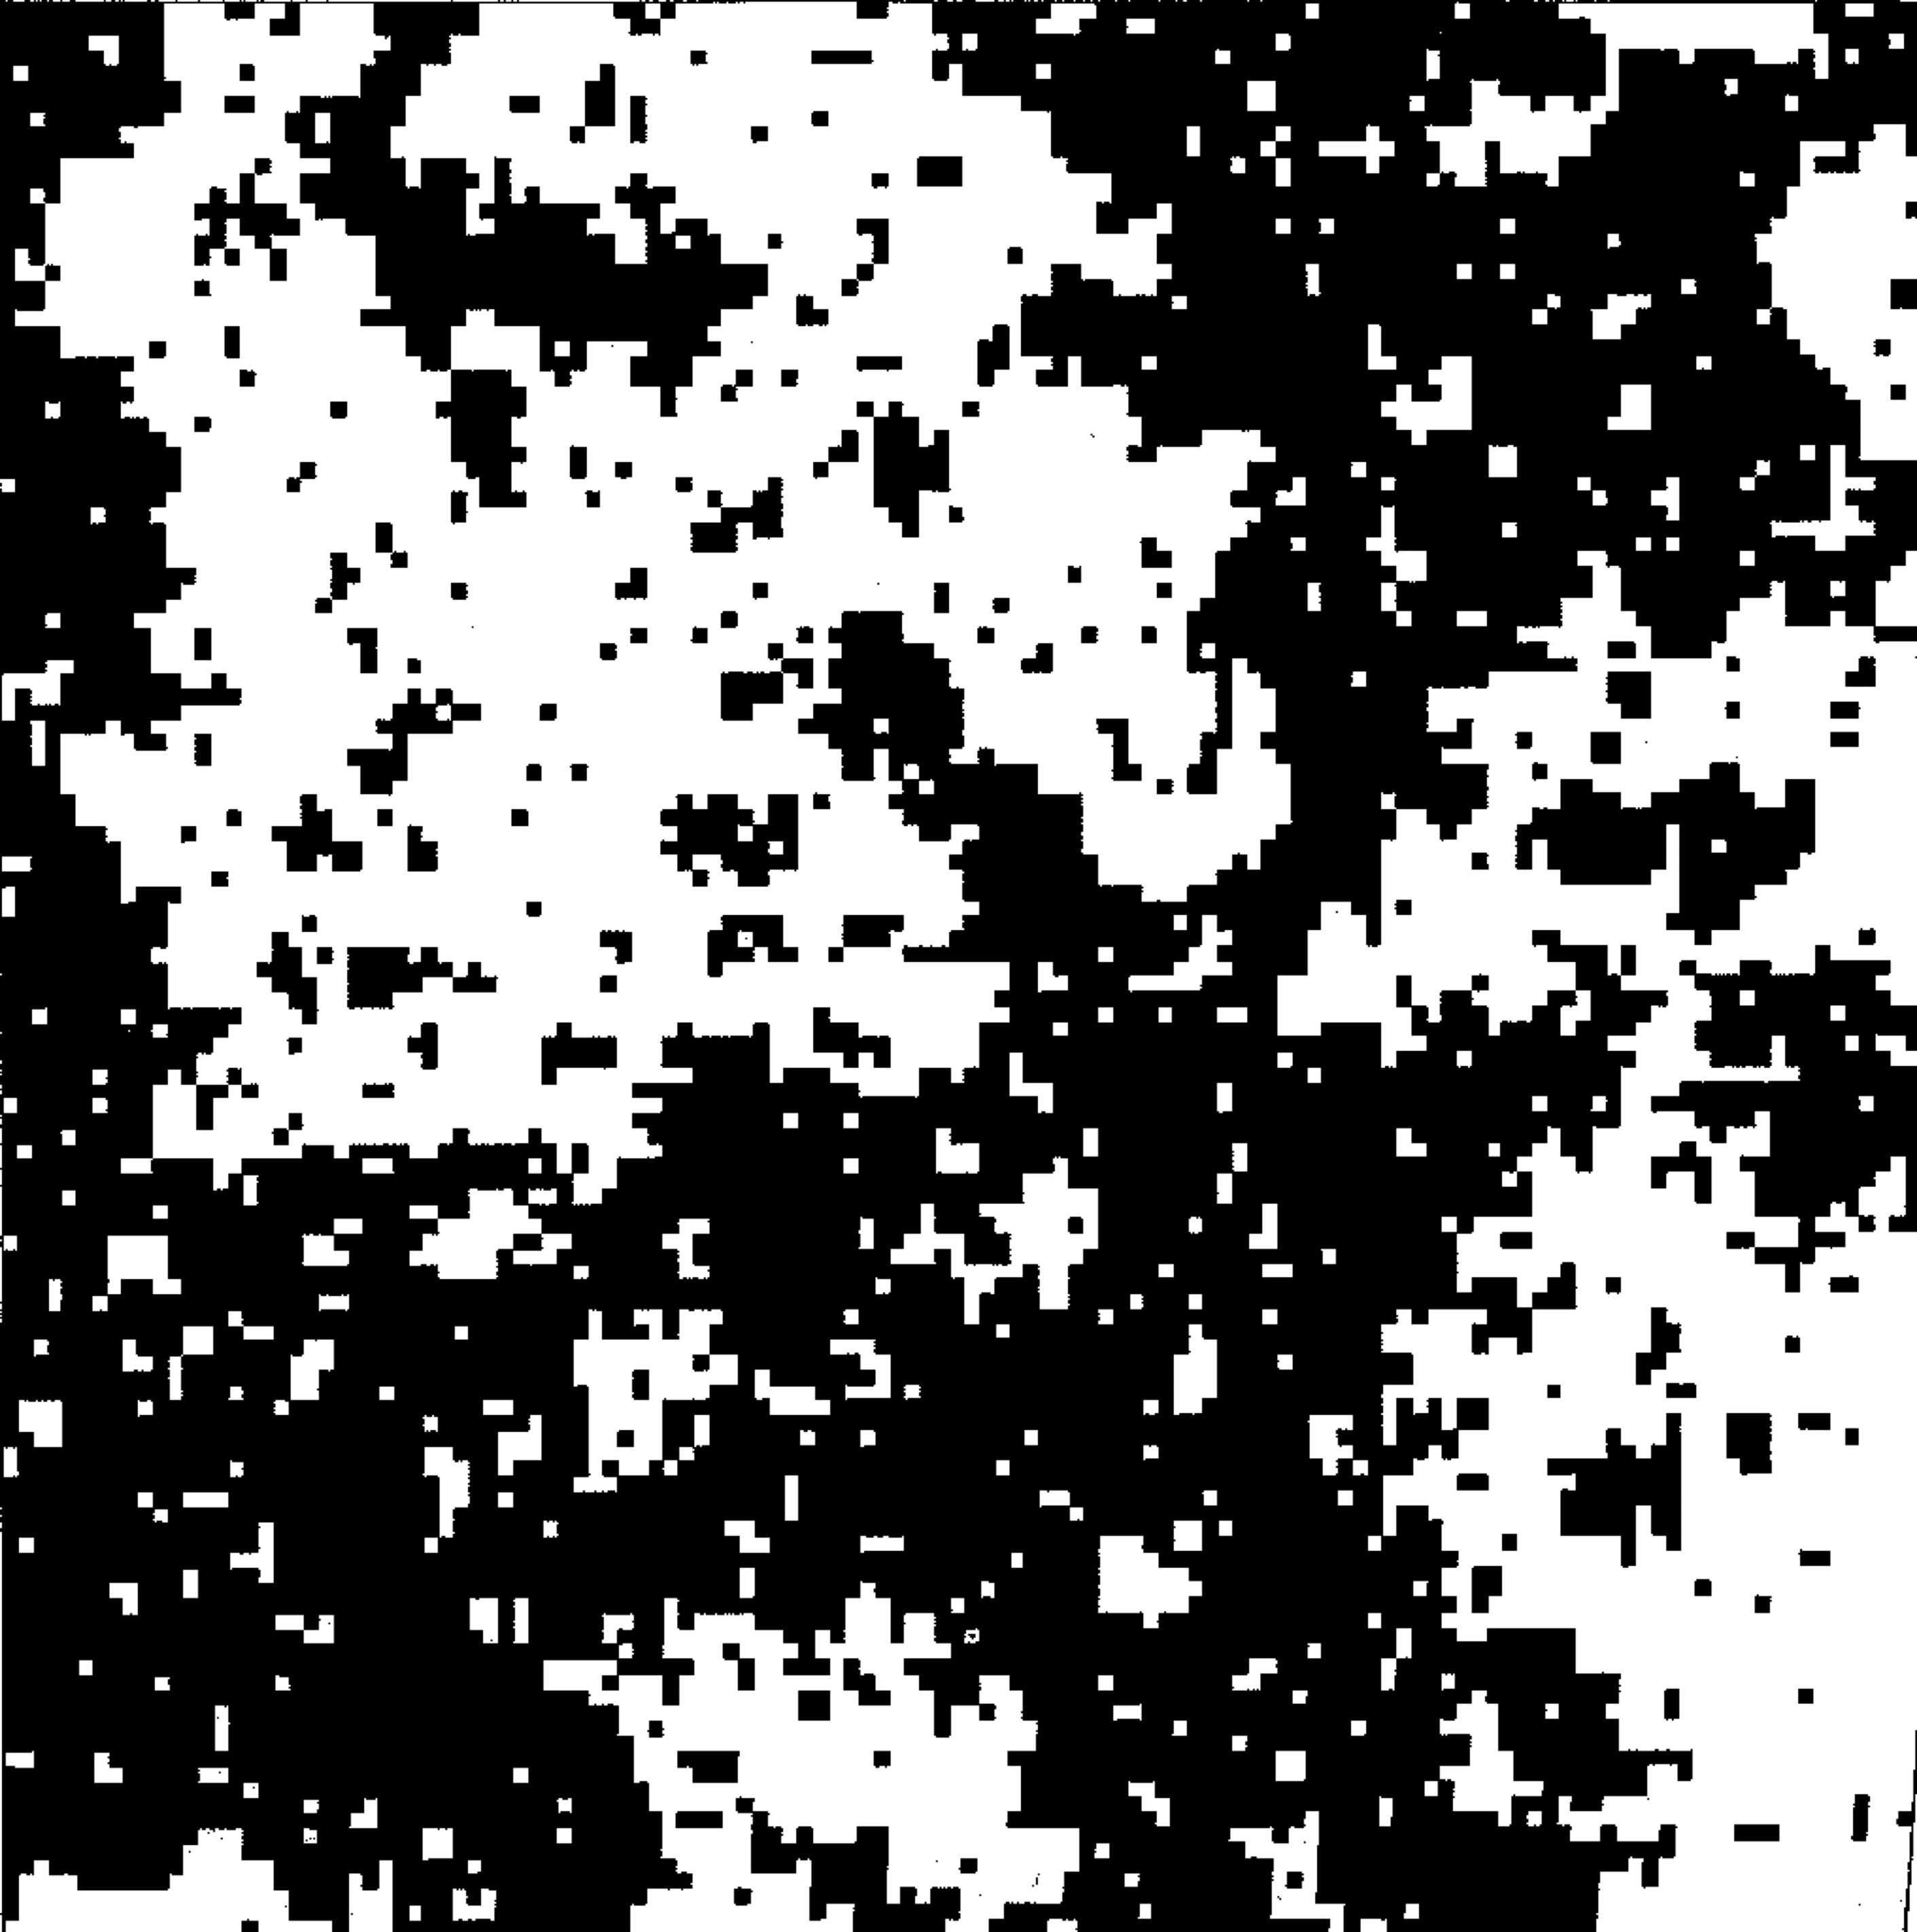
\includegraphics[keepaspectratio]{phase-transitions/Figs/crit.png}}

}

\subcaption{\label{fig-ssb}\(T=T_c\)}

\end{minipage}%
%
\begin{minipage}{0.33\linewidth}

\centering{

\pandocbounded{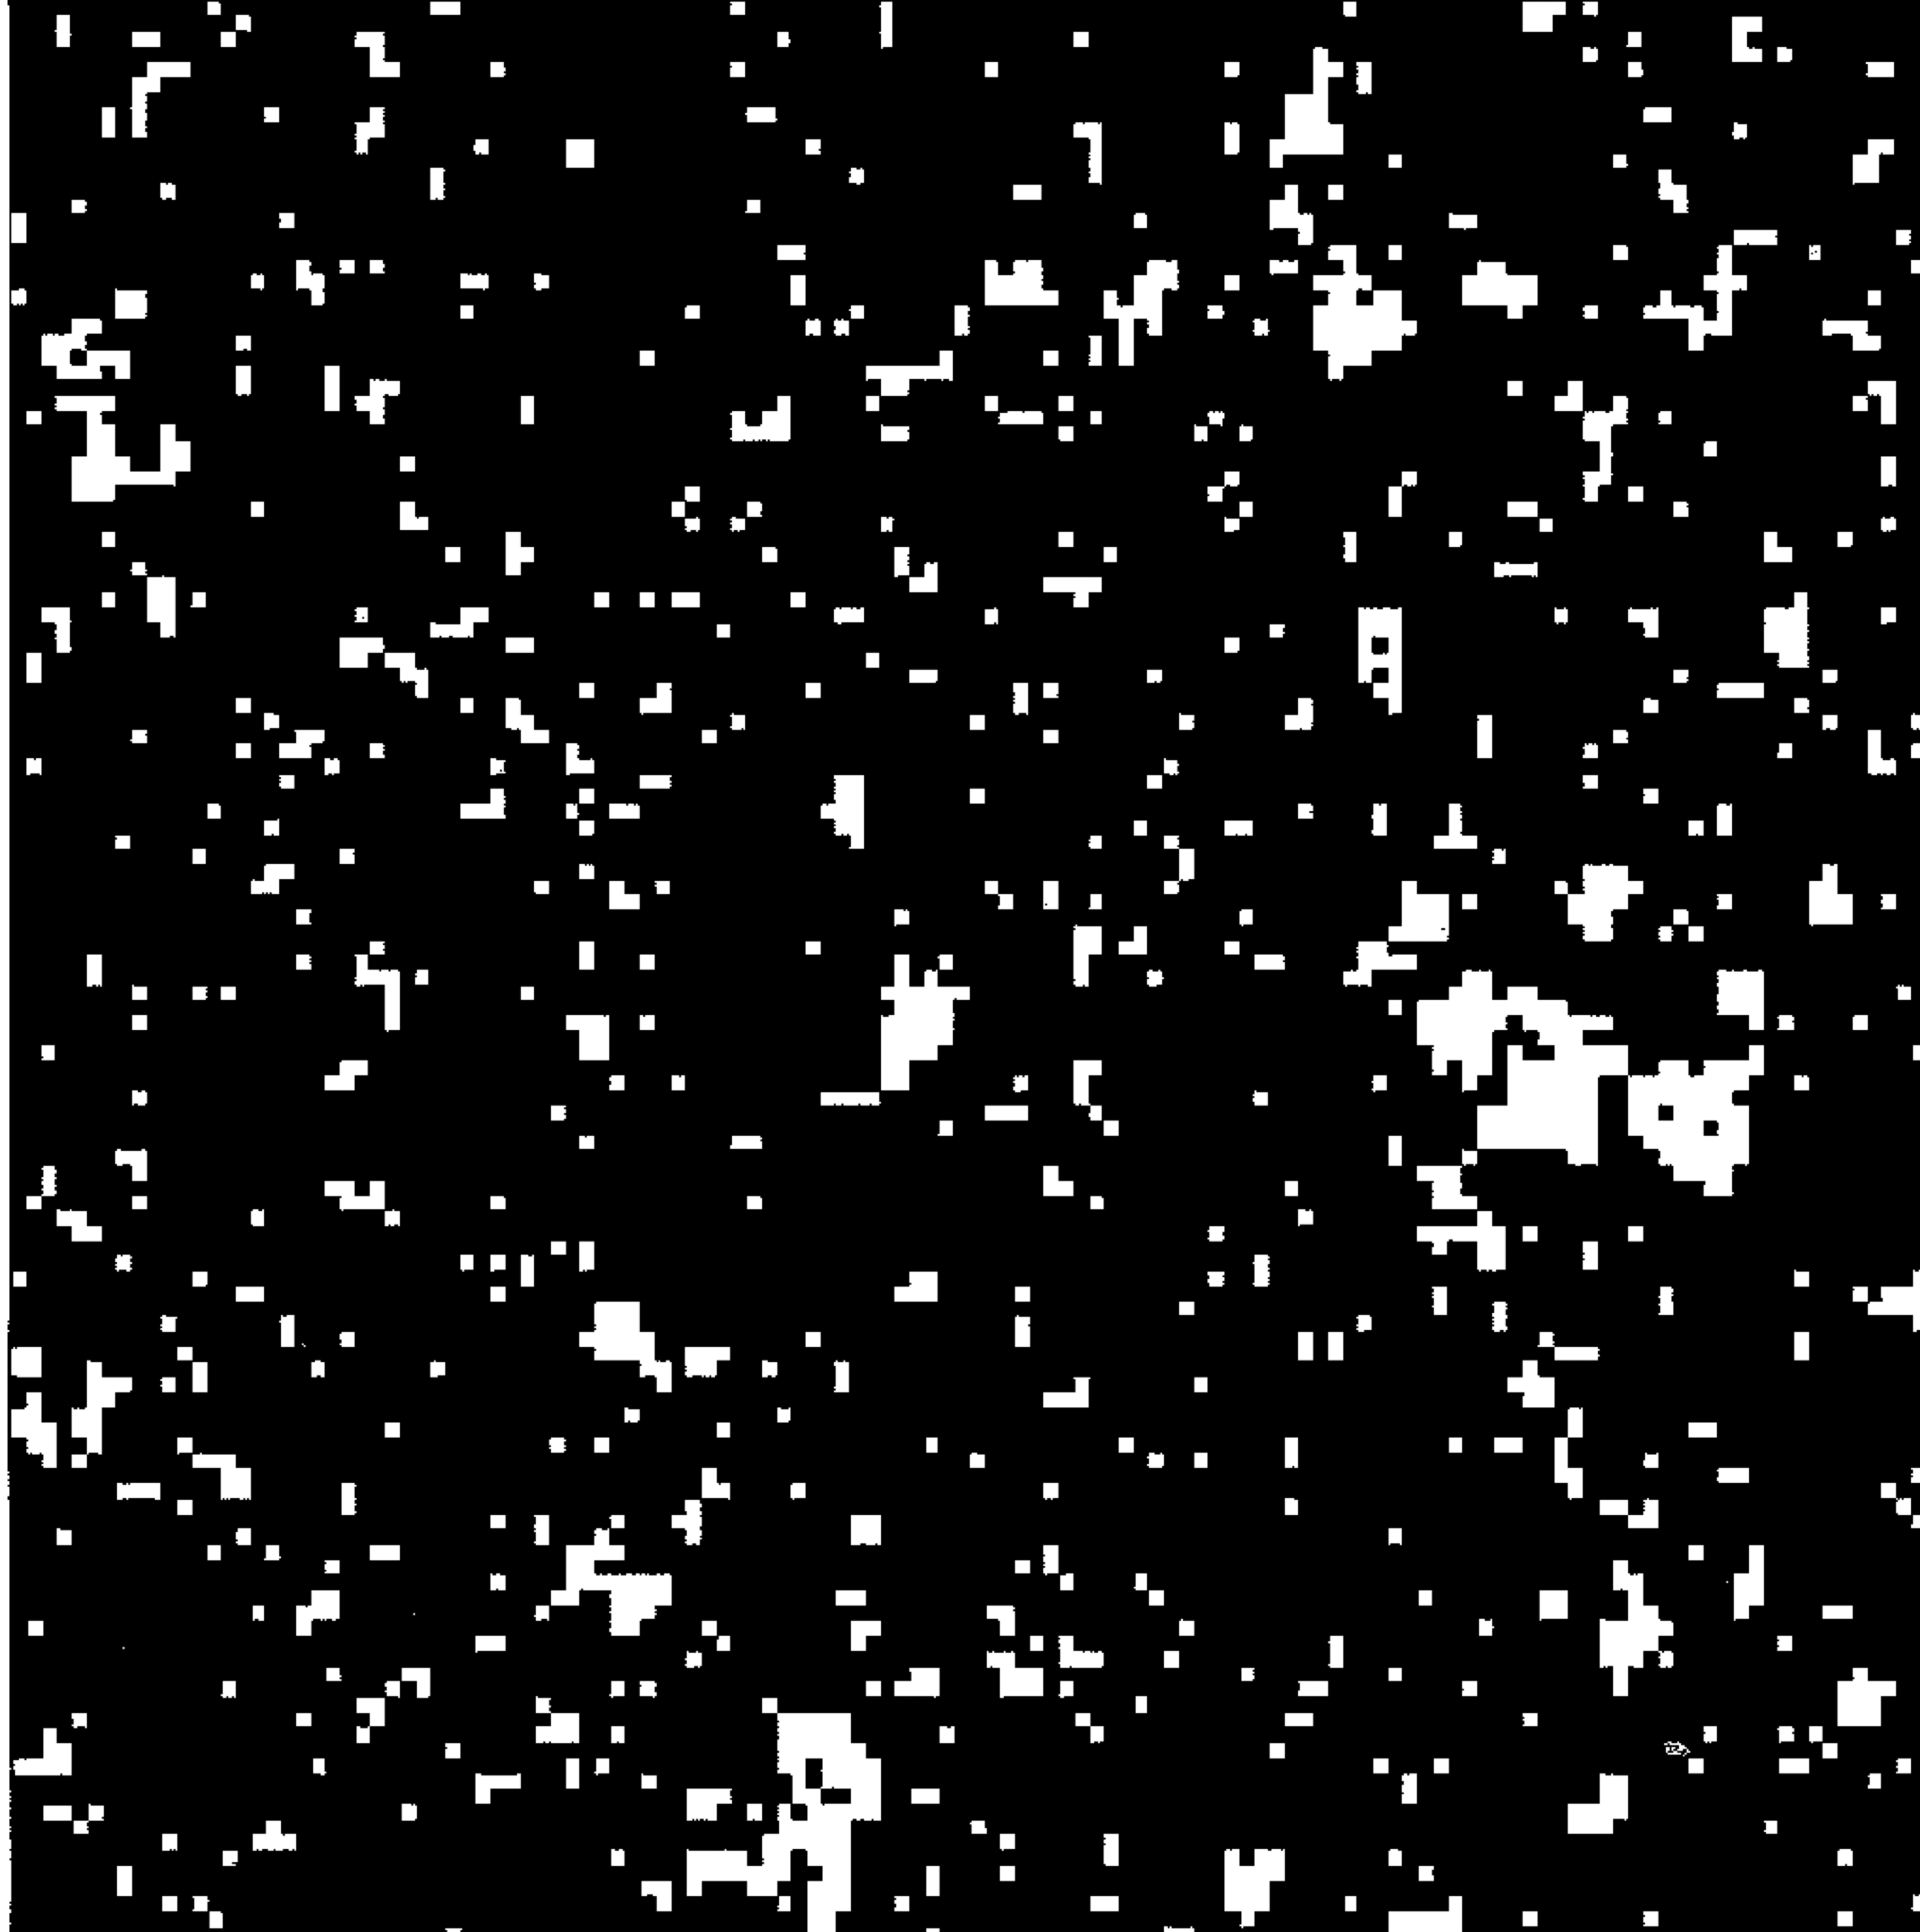
\includegraphics[keepaspectratio]{phase-transitions/Figs/subcrit.png}}

}

\subcaption{\label{fig-ssc}\(T=0.95T_c\)}

\end{minipage}%

\caption{\label{fig-snapshots}Configurations of the 2d Ising model. The
patterns depict typical arrangements of the spins (white=+1, black=−1)
generated in a computer simulation of the Ising model on a square
lattice of \(N=512\) sites, at temperatures (from left to right) of
\(T= 1.2T_c\), \(T=T_c\), and \(T=0.95T_c\). In each case only a portion
of the system containing \(128\) sites in shown. The typical island size
is a measure of the correlation length \(\xi\): the excess of black over
white (below \(T_c\) is a measure of the order parameter.}

\end{figure}%

\href{https://physics.weber.edu/schroeder/software/demos/isingmodel.html}{An
interactive Monte Carlo simulation of the Ising model} demonstrates the
phenomenology, By altering the temperature you will be able to observe
for yourself how the typical spin arrangements change as one traverses
the critical region. Pay particular attention to the configurations near
the critical point. They have very interesting properties. We will
return to them later!

Although the 2-d Ising model may appear at first sight to be an
excessively simplistic portrayal of a real magnetic system, critical
point universality implies that many physical observables such as
critical exponents are not materially influenced by the actual nature of
the microscopic interactions. The Ising model therefore provides a
simple, yet \emph{quantitatively} accurate representation of the
critical properties of a whole range of real magnetic (and indeed fluid)
systems. This universal feature of the model is largely responsible for
its ubiquity in the field of critical phenomena. We shall explore these
ideas in more detail later in the course.

\section{Exact solutions: the one dimensional Ising
chain}\label{exact-solutions-the-one-dimensional-ising-chain}

One might well ask why the 2D Ising model is the simplest model to
exhibit a phase transition. What about the one-dimensional Ising model
(ie. spins on a line)? In fact in one dimension, the Ising model can be
solved exactly. It turns out that the system is paramagnetic for all
\(T>0\), so there is no phase transition at any finite temperature. To
see this, consider the ground state of the system in zero external
field. This will have all spins aligned the same way (say up), and hence
be ferromagnetic. Now consider a configuration with a various ``domain
walls'' dividing spin up and spin down regions:

\begin{figure}

\centering{

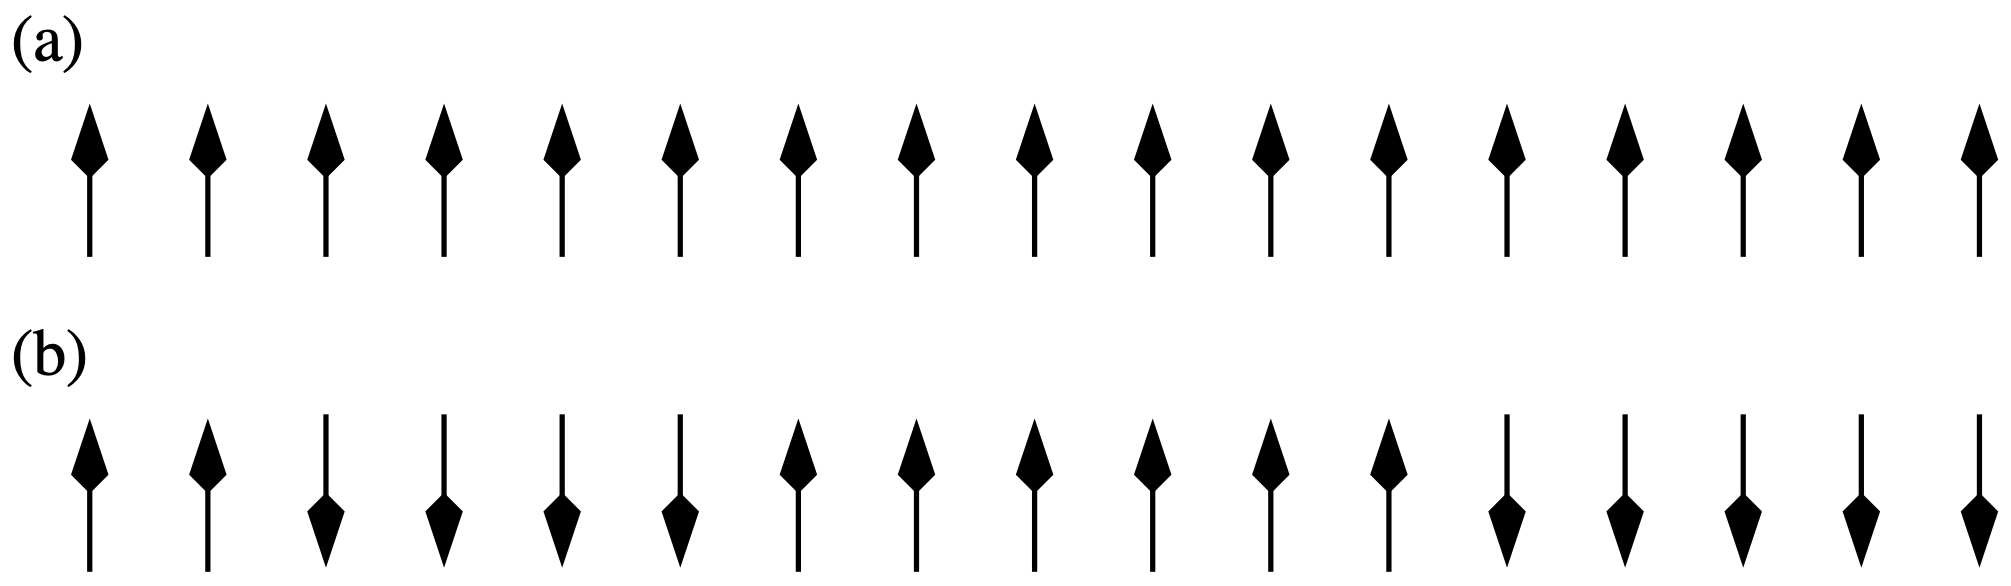
\includegraphics[width=0.8\linewidth,height=\textheight,keepaspectratio]{phase-transitions/Figs/chain.png}

}

\caption{\label{fig-isingchain}(a) Schematic of an Ising chain at
\(T=0\). (b) At a small finite temperature the chain is split into
domains of spins ordered in the same direction. Domains are separated by
notional domain ``walls'', which cost energy \(\Delta=2J\). Periodic
boundary conditions are assumed.}

\end{figure}%

Instead of considering the underlying spin configurations, we shall
describe the system in terms of the statistics of its domain walls. The
energy cost of a wall is \(\Delta = 2J\), independent of position.
Domain walls can occupy the bonds of the lattice, of which there are
\(N-1\). Moreover, the walls are noninteracting, except that you cannot
have two of them on the same bond. (Check through these ideas if you are
unsure.)

In this representation, the partition function involves a count over all
possible domain wall arrangements. Since the domain walls are non
interacting (eg it doesn't cost energy for one to move along the chain)
they can be treated as independent. Independent contributions to the
partition function simply multiply. So we can calculate \(Z\) by
considering the partition function associated with a single domain wall
being present or absent on some given bond, and then simply raise to the
power of the number of bonds:

\[Z=Z_1^{N-1}\]

where

\[Z_1=e^{\beta J} + e^{\beta (J-\Delta)}=e^{\beta J}(1+e^{-\beta\Delta})\]
is the domain wall partition function for a single bond and represent
the sum over the two possible states: domain wall absent or present.
Then the free energy per bond of the system is

\[\beta f\equiv \beta F/(N-1)=-\ln Z_1=-\beta J-\ln(1+e^{-\beta\Delta})\]

The first term on the RHS is simply the energy per spin of the
ferromagnetic (ordered) phase, while the second term arises from the
free energy of domain walls. Clearly for any finite temperature (ie. for
\(\beta<\infty\)), this second term is finite and negative. Hence the
free energy will always be lowered by having a finite concentration of
domain walls in the system. Since these domain walls disorder the
system, leading to a zero average magnetisation, the 1D system is
paramagnetic for all finite temperatures. \emph{Exercise}: Explain why
this argument works only in 1D.

The animation below lets you see qualitatively how the typical number of
domain walls varies with temperature. If you'd lke to explore more
quantitatively, a python code performing a Monte Carlo simulation is
available. You will learn about Monte Carlo simulation in the coursework
and in later parts of the course.

\begin{Shaded}
\begin{Highlighting}[]
\CommentTok{\#Monte Carlo simulation of the 1d Ising chain with periodic bounary conditions}
\ImportTok{import}\NormalTok{ numpy }\ImportTok{as}\NormalTok{ np}
\ImportTok{import}\NormalTok{ matplotlib.pyplot }\ImportTok{as}\NormalTok{ plt}
\ImportTok{from}\NormalTok{ matplotlib.animation }\ImportTok{import}\NormalTok{ FuncAnimation}
\ImportTok{from}\NormalTok{ matplotlib.widgets }\ImportTok{import}\NormalTok{ Slider}

\CommentTok{\# Number of spins}
\NormalTok{N }\OperatorTok{=} \DecValTok{20} 

\CommentTok{\# Initialize spins (+1 or {-}1)}
\NormalTok{spins }\OperatorTok{=}\NormalTok{ np.random.choice([}\OperatorTok{{-}}\DecValTok{1}\NormalTok{, }\DecValTok{1}\NormalTok{], size}\OperatorTok{=}\NormalTok{N)}

\CommentTok{\# Initial temperature}
\NormalTok{T }\OperatorTok{=} \FloatTok{2.0}

\CommentTok{\# Set up figure and axis for the spins}
\NormalTok{fig, ax }\OperatorTok{=}\NormalTok{ plt.subplots(figsize}\OperatorTok{=}\NormalTok{(}\DecValTok{10}\NormalTok{, }\DecValTok{2}\NormalTok{))}
\NormalTok{plt.subplots\_adjust(bottom}\OperatorTok{=}\FloatTok{0.25}\NormalTok{)  }\CommentTok{\# make room for slider}
\NormalTok{ax.set\_xlim(}\OperatorTok{{-}}\FloatTok{0.5}\NormalTok{, N }\OperatorTok{{-}} \FloatTok{0.5}\NormalTok{)}
\NormalTok{ax.set\_ylim(}\OperatorTok{{-}}\DecValTok{1}\NormalTok{, }\DecValTok{1}\NormalTok{)}
\NormalTok{ax.axis(}\StringTok{\textquotesingle{}off\textquotesingle{}}\NormalTok{)}

\CommentTok{\# Create text objects for each spin}
\NormalTok{texts }\OperatorTok{=}\NormalTok{ []}
\ControlFlowTok{for}\NormalTok{ i }\KeywordTok{in} \BuiltInTok{range}\NormalTok{(N):}
\NormalTok{    arrow }\OperatorTok{=} \StringTok{\textquotesingle{}↑\textquotesingle{}} \ControlFlowTok{if}\NormalTok{ spins[i] }\OperatorTok{==} \DecValTok{1} \ControlFlowTok{else} \StringTok{\textquotesingle{}↓\textquotesingle{}}
\NormalTok{    t }\OperatorTok{=}\NormalTok{ ax.text(i, }\DecValTok{0}\NormalTok{, arrow, fontsize}\OperatorTok{=}\DecValTok{24}\NormalTok{, ha}\OperatorTok{=}\StringTok{\textquotesingle{}center\textquotesingle{}}\NormalTok{, va}\OperatorTok{=}\StringTok{\textquotesingle{}center\textquotesingle{}}\NormalTok{)}
\NormalTok{    texts.append(t)}

\KeywordTok{def}\NormalTok{ update(frame):}
    \CommentTok{"""Perform Metropolis updates over all spins, then refresh display."""}
    \KeywordTok{global}\NormalTok{ spins, T}
    \ControlFlowTok{for}\NormalTok{ \_ }\KeywordTok{in} \BuiltInTok{range}\NormalTok{(N):}
\NormalTok{        i }\OperatorTok{=}\NormalTok{ np.random.randint(N)}
\NormalTok{        left }\OperatorTok{=}\NormalTok{ spins[(i }\OperatorTok{{-}} \DecValTok{1}\NormalTok{) }\OperatorTok{\%}\NormalTok{ N]}
\NormalTok{        right }\OperatorTok{=}\NormalTok{ spins[(i }\OperatorTok{+} \DecValTok{1}\NormalTok{) }\OperatorTok{\%}\NormalTok{ N]}
\NormalTok{        deltaE }\OperatorTok{=} \DecValTok{2} \OperatorTok{*}\NormalTok{ spins[i] }\OperatorTok{*}\NormalTok{ (left }\OperatorTok{+}\NormalTok{ right)}
        \CommentTok{\# Metropolis criterion ensures configurations appear with the correct Boltzmann probability}
        \ControlFlowTok{if}\NormalTok{ deltaE }\OperatorTok{\textless{}} \DecValTok{0} \KeywordTok{or}\NormalTok{ np.random.rand() }\OperatorTok{\textless{}}\NormalTok{ np.exp(}\OperatorTok{{-}}\NormalTok{deltaE }\OperatorTok{/}\NormalTok{ T):}
\NormalTok{            spins[i] }\OperatorTok{*=} \OperatorTok{{-}}\DecValTok{1}
    \CommentTok{\# Update arrows on screen}
    \ControlFlowTok{for}\NormalTok{ idx, t }\KeywordTok{in} \BuiltInTok{enumerate}\NormalTok{(texts):}
\NormalTok{        t.set\_text(}\StringTok{\textquotesingle{}↑\textquotesingle{}} \ControlFlowTok{if}\NormalTok{ spins[idx] }\OperatorTok{==} \DecValTok{1} \ControlFlowTok{else} \StringTok{\textquotesingle{}↓\textquotesingle{}}\NormalTok{)}
    \ControlFlowTok{return}\NormalTok{ texts}

\CommentTok{\# Create the animation with caching disabled and blit turned off}
\NormalTok{ani }\OperatorTok{=}\NormalTok{ FuncAnimation(}
\NormalTok{    fig,}
\NormalTok{    update,}
\NormalTok{    interval}\OperatorTok{=}\DecValTok{200}\NormalTok{,}
\NormalTok{    blit}\OperatorTok{=}\VariableTok{False}\NormalTok{,}
\NormalTok{    cache\_frame\_data}\OperatorTok{=}\VariableTok{False}
\NormalTok{)}

\CommentTok{\# Add a temperature slider}
\NormalTok{ax\_T }\OperatorTok{=}\NormalTok{ plt.axes([}\FloatTok{0.2}\NormalTok{, }\FloatTok{0.1}\NormalTok{, }\FloatTok{0.6}\NormalTok{, }\FloatTok{0.03}\NormalTok{], facecolor}\OperatorTok{=}\StringTok{\textquotesingle{}lightgray\textquotesingle{}}\NormalTok{)}
\NormalTok{slider\_T }\OperatorTok{=}\NormalTok{ Slider(ax\_T, }\StringTok{\textquotesingle{}Temperature T\textquotesingle{}}\NormalTok{, }\FloatTok{0.1}\NormalTok{, }\FloatTok{5.0}\NormalTok{, valinit}\OperatorTok{=}\NormalTok{T)}

\KeywordTok{def}\NormalTok{ on\_T\_change(val):}
    \CommentTok{"""Callback to update T when the slider changes."""}
    \KeywordTok{global}\NormalTok{ T}
\NormalTok{    T }\OperatorTok{=}\NormalTok{ val}

\NormalTok{slider\_T.on\_changed(on\_T\_change)}

\CommentTok{\# Show the plot (ani is kept in scope so it won\textquotesingle{}t be deleted)}
\NormalTok{plt.show()}
\end{Highlighting}
\end{Shaded}

\phantomsection\label{ising}

Temperature T =

2.0

\subsection{More general 1D spins systems: transfer matrix
method}\label{more-general-1d-spins-systems-transfer-matrix-method}

Generally speaking one-dimensional systems lend themselves to a degree
of analytic tractability not found in most higher dimensional models.
Indeed for the case of a 1-d assembly of \(N\) spins each having \(m\)
discrete energy states, and in the presence of a magnetic field, it is
possible to reduce the evaluation of the partition function to the
calculation of the eigenvalues of a matrix--the so called transfer
matrix.

Let us start by assuming that the assembly has cyclic boundary
conditions, then the total energy of configuration \(\{s\}\) is \[
\begin{aligned}
{\cal H}(\{s\})=&-\sum_{i=1}^N (J s_i s_{i+1}+Hs_i)\\
\:=&-\sum_{i=1}^N (J s_i s_{i+1}+H(s_i+s_{i+1})/2)\\
\:=&\sum_{i=1}^N E(s_i,s_{i+1})
\end{aligned}
\]

where we have defined
\(E(s_i,s_{i+1})=-J s_i s_{i+1}-H(s_i+s_{i+1})/2\).

Now the partition function may be written

\begin{equation}\phantomsection\label{eq-Vs}{\begin{aligned}
Z_N =& \sum_{\{s\}}\exp\left(-\beta {\cal H}(\{s\})\right)\nonumber \\
 =&\sum_{\{s\}}\exp\left(-\beta[E(s_1,s_2)+E(s_2,s_3)+....E(s_N,s_1)]\right) \nonumber\\
 =&\sum_{\{s\}}\exp\left(-\beta E(s_1,s_2)\right)\exp\left(-\beta E(s_2,s_3)\right)....\exp\left(-\beta E(s_N,s_1)\right) \nonumber\\
=&\sum_{i,j,...,l=1}^m V_{ij}V_{jk}...V_{li} 
\end{aligned}}\end{equation}

where the \(V_{ij}=\exp(-\beta E_{ij})\) are elements of an
\(m \times m\) matrix \({\bf V}\), known as the transfer matrix
(\(i,j,k\) etc are dummy indices that run over the matrix elements). You
should see that the sum over the product of matrix elements picks up all
the terms in the partition function and therefore Equation~\ref{eq-Vs}
is an alternative way of writing the partition function.

The reason it is useful to transform to a matrix representation is that
it transpires that the sum over the product of matrix elements in
Equation~\ref{eq-Vs} is simply just the trace of \({\bf V}^N\) (check
this yourself for a short periodic chain), given by the sum of its
eigenvalues:-

\[Z_N=\lambda_1^N+\lambda_2^N+...\lambda_m^N\] For very large \(N\),
this expression simplifies further because the largest eigenvalue
\(\lambda_1\) dominates the behaviour since \((\lambda_2/\lambda_1)^N\)
vanishes as \(N\rightarrow \infty\). Consequently in the thermodynamic
limit one may put \(Z_N=\lambda_1^N\) and the problem reduces to
identifying the largest eigenvalue of the transfer matrix.

Specializing to the case of the simple Ising model in the presence of an
applied field \(H\), the transfer matrix takes the form

\[{\bf V}(H)=\left(
\begin{array}{cc}
e^{\beta(J+H)} & e^{-\beta J} \\
e^{-\beta J}   & e^{\beta(J-H)}
\end{array} \right)\]

This matrix has two eigenvalues which can be readily calculated in the
usual fashion as the roots of the characteristic polynomial
\(|{\bf V}-\lambda{\bf I}|\). They are

\[\lambda_{\pm}=e^{\beta J}\cosh(\beta H) \pm \sqrt{e^{2\beta J}\sinh^2\beta H+e^{-2\beta J}}.\]

Hence the free energy per spin \(f=-k_BT\ln \lambda_+\) is

\[f=-k_BT\ln \left[e^{\beta J}\cosh(\beta H) + \sqrt{e^{2\beta J}\sinh^2\beta H+e^{-2\beta J}}\right].\]

The Ising model in 2D can also be solved exactly, as was done by Lars
Onsager in 1940. The solution is extremely complicated and is regarded
as one of the pinnacles of statistical mechanics. In 3D no exact
solution is known.

\chapter*{Tools for understanding complex disordered
matter}\label{tools-for-understanding-complex-disordered-matter}
\addcontentsline{toc}{chapter}{Tools for understanding complex
disordered matter}

\markboth{Tools for understanding complex disordered matter}{Tools for
understanding complex disordered matter}

Complex disordered systems are composed of an enormous number of
interacting components---typically on the order of \(\sim 10^{23}\).
These interactions can lead to fascinating emergent behaviour, but they
also render the systems analytically intractable; it is clearly
impossible to solve Newton's equations for such vast numbers of
particles. To address this difficulty, we turn to Statistical Mechanics,
which you first encountered in your second year. Statistical Mechanics
provides the essential framework for connecting the microscopic
behaviour of individual constituents with the macroscopic thermodynamic
and dynamical properties of the system as a whole.

In this section, we will revisit and expand upon key concepts relevant
to our discussion, with particular emphasis on the \textbf{free
energy}---a central quantity that captures the balance between energy
minimisation and entropy maximisation in determining the system's
equilibrium state. If any of these ideas feel unfamiliar, you may find
it useful to revise the Statistical Mechanics material from your Year 2
\emph{Thermal Physics} course notes.

\section*{Ensembles and free
energies}\label{ensembles-and-free-energies}
\addcontentsline{toc}{section}{Ensembles and free energies}

\markright{Ensembles and free energies}

Statistical mechanics can be formulated in a variety of ensembles
reflecting the relationship between the system and its environment. In
what follows we summarise the formalism, focussing on the case of a
particle fluid. Analogous equations apply to lattice spin models (see
lectures and the book by Yeomans). Key ensembles are:

\subsection*{Microcanonical ensemble}\label{microcanonical-ensemble}
\addcontentsline{toc}{subsection}{Microcanonical ensemble}

Applies to a system of \(N\) particles (or spins) in a fixed volume
\(V\) having adiabatic walls so that the internal energy \(E\) is
constant. Denoted as constant-\(NVE\). Let \(\Omega\) be the number of
(micro)states having the prescribed energy:

\[
\Omega=\sum_\textrm{all states having energy E}
\]

Thermodynamically, the states favored in the canonical ensemble are
those that maximise the entropy:

\[
S=k_B\ln \Omega\: .
\]

where \(k_B\) is Boltzmann's constant The microcanonical ensemble is
useful for defining the entropy, but is little used in practice.

\subsection*{Canonical ensemble}\label{sec-canonical}
\addcontentsline{toc}{subsection}{Canonical ensemble}

Applies to a system of \(N\) particles in a fixed volume \(V\) and
coupled to a heat bath at temperature \(T\). Denoted as
constant-\(NVT\). A central quantity is the \emph{partition function}

\begin{equation}\phantomsection\label{eq-ZNVT}{
Z_{NVT}=\sum_\textrm{ all states i}e^{-\beta E_i},~~~~~\beta=1/(k_BT)
}\end{equation} which is a weighted sum over the states. The partition
function provides the normalisation constant in the probability of
finding the system in a given state \(i\).

\begin{equation}\phantomsection\label{eq-Pi}{
P_i=\frac{e^{-\beta E_i}}{Z_{NVT}}.
}\end{equation}

The states favored in the canonical ensemble are those that minimise the
free energy:

\[
F_{NVT}=-\beta^{-1}\ln Z_{NVT}\:.
\]

\(F_{NVT}\) is known as the Helmholtz free energy. Thermodynamics also
supplies a relation for the Helmholtz free energy:

\[
F_{NVT}=E-TS\:,
\] where \(E\) is the average internal energy. In minimising the free
energy, the system strikes a compromise between low energy and high
entropy. The temperature plays the role of arbiter, favouring high
entropy at high \(T\), and low energy at low \(T\). The canonical
ensemble is usually used to describe systems such as magnets, or a fluid
held at constant volume. It is the ensemble we shall use most in this
course.

\subsection*{Grand canonical ensemble}\label{sec-grandcanonical}
\addcontentsline{toc}{subsection}{Grand canonical ensemble}

Applies to a system with a variable number of particle in a fixed volume
\(V\) coupled to both a heat bath at temperature \(T\) and a particle
reservoir with chemical potential \(\mu\) (which is the field conjugate
to \(N\)). Denoted as constant-\(\mu VT\).

The corresponding partition function is a weighted superset of the
canonical one

\[
Z_{\mu VT}=\sum_{N=0}^\infty e^{\beta\mu N}Z_{NVT}
\] and a state probability analogous to Equation~\ref{eq-Pi} holds. One
can recast this in a form similar to Equation~\ref{eq-ZNVT}:

\begin{equation}\phantomsection\label{eq-ZmuVT}{
Z_{\mu VT}=\sum_{N=0}^\infty\:\sum_\textrm{all~states~i}e^{-\beta {\cal H}_i},
}\end{equation} where \({\cal H}_i=E_i-\mu N\) is the form of the
Hamiltonian in the grand canonical ensemble.

Statistically, the states favored in the grand canonical ensemble are
those that minimise the free energy:

\[
F_{\mu VT}=-\beta^{-1}\ln Z_{\mu VT}
\] \(F_{\mu VT}\) is known as the grand potential. It can also be
derived from thermodynamics, from which one finds

\[
F_{\mu VT}=E-TS-\mu N=-pV,
\] where \(p\) is the pressure.

The grand canonical ensemble is usually used to describe systems such as
fluid connected to a particle reservoir. Sometimes for a magnet we
consider the effects of an applied magnetic field, which is analogous to
working in the grand canonical ensemble: the magnetic field (which is
conjugate to the magnetisation) plays a similar role to the chemical
potential in a fluid.

\subsection*{Isothermal-isobaric
ensemble}\label{isothermal-isobaric-ensemble}
\addcontentsline{toc}{subsection}{Isothermal-isobaric ensemble}

Applies to a system with a fixed number of particles \(N\) that is
coupled to a heat bath at temperature \(T\) and a reservoir that exerts
a constant pressure \(p\) which allows the sample volume to fluctuate.
Denoted as constant-\(NpT\).

The corresponding partition function is a weighted superset of the
canonical one

\[
Z_{NpT}=\int_0^\infty dV  e^{-\beta p V}Z_{NVT}
\] or \begin{equation}\phantomsection\label{eq-ZNpT}{
Z_{NpT}=\int_0^\infty dV\:\sum_\textrm{i}e^{-\beta {\cal H}_i},
}\end{equation} where \({\cal H}_i=E_i+pV\) is the form of the
Hamiltonian in the constant-\(NpT\) ensemble. Again a state probability
analogous to Equation~\ref{eq-Pi} holds.

Statistically, the states favored in the constant-\(NpT\) ensemble are
those that minimise the free energy:

\[
F_{NpT}=-\beta^{-1}\ln Z_{NpT}
\] \(F_{NpT}\) is known as the \emph{Gibb's free energy} (often denoted
\(G\)). It can also be derived from thermodynamics, from which one finds

\[
F_{NpT}=E-TS+pV=\mu N
\]

The constant-\(NpT\) ensemble is usually used to describe systems such
as a fluid subject to a variable pressure, or a magnet coupled to a
magnetic field \(H\). In the latter case the quantity \(HM\) plays the
role of \(pV\) and

\[
F_{NpT}=E-TS-MH\:,
\] with \(M\) the total magnetisation.

\section*{From free energies to
observables}\label{from-free-energies-to-observables}
\addcontentsline{toc}{section}{From free energies to observables}

\markright{From free energies to observables}

Free energies are not directly observable quantities. However, all
physical observables can be expressed in terms of \emph{derivatives} of
the free energy. One can derive the appropriate relations either from
Thermodynamics, or the corresponding statistical mechanics (Revise your
year-2 Thermal Physics notes on this if necessary). As an example let us
consider a fluid in the isothermal-isobaric ensemble for which the
appropriate free energy is \(F_{NpT}=E-TS+pV\), and where the volume
fluctuates in response to the prescribed pressure. We shall seek an
expression for the average volume in terms of the free energy. First
lets us take the thermodynamic route. Differentiating the free energy
and applying the chain rule we have:

\[
dF=dE-TdS-sdT+pdV+VdP\:.
\] But from the first law of thermodynamics, \(dE=TdS-pdV\), so

\[
dF=-SdT+Vdp\:,
\] and rearranging yields \[
V=\left(\frac{\partial F}{\partial p}\right)_T\:.
\]

We can now show that this result is consistent with the definition of
\(F_{NpT}\) in terms of the partition function. Write

\[
Z_{NpT}=\int_0^\infty dV  e^{-\beta p V}Z_{NVT}=\int_0^\infty dV\sum_{all~states~i}e^{-\beta (p V_i+E_i)}
\]

Then

\begin{align}
\left(\frac{\partial F}{\partial p}\right)_T
&= -\frac{1}{\beta} \left(\frac{\partial \ln Z_{NpT}}{\partial p}\right)_T \\
&= -\frac{1}{\beta} \frac{1}{Z_{NpT}} \frac{\partial Z_{NpT}}{\partial p} \\
&= -\frac{1}{\beta} \frac{1}{Z_{NpT}} \int_0^\infty dV \int_{\text{all states}} (-\beta V) e^{-\beta (p V + E)} \\
&= \langle V \rangle_T \,.
\end{align}

where in the last step we have used the fact that the probability of a
state is defined to be \(e^{-\beta (p V_i+E_i)}/Z_{NpT}\).

\emph{Exercise}. Repeat these manipulations to find an expression for
the mean particle number \(N\) in the grand canonical ensemble

\begin{tcolorbox}[enhanced jigsaw, colframe=quarto-callout-caution-color-frame, colback=white, bottomtitle=1mm, rightrule=.15mm, arc=.35mm, toptitle=1mm, leftrule=.75mm, opacityback=0, breakable, bottomrule=.15mm, colbacktitle=quarto-callout-caution-color!10!white, left=2mm, titlerule=0mm, toprule=.15mm, opacitybacktitle=0.6, coltitle=black, title=\textcolor{quarto-callout-caution-color}{\faFire}\hspace{0.5em}{Solution}]

In the grand canonical ensemble (GCE), the relevant free energy is

\[
F_{\mu VT} = E - TS - \mu N
\]

From the first law of thermodynamics changes in the internal energy are
given by:

\[
dE = TdS - PdV + \mu dN=TdS+\mu dN
\] where we have used the fact that \(V\) is fixed in the GCE, so
\(dV=0\).

Differentiating \(F_{\mu VT}\):

\[
dF_{\mu VT} = dE - TdS - SdT - \mu dN - N d\mu
= -S dT - N d\mu
\] where for the last equality we have substitued for \(dE\) from above.

Thus \[
\left( \frac{\partial F_{\mu VT}}{\partial \mu} \right)_{T, V} = -N
\quad \Rightarrow \quad
\langle N \rangle = -\left( \frac{\partial F_{\mu VT}}{\partial \mu} \right)_{T, V}
\]

Now consider the statistical mechanics route to calculate
\(\langle N\rangle\):

\[
Z_{\mu V T} = \sum_{N=0}^{\infty} \sum_{\text{states}} e^{-\beta (E_{N,i} - \mu N)}
\]

The grand potential (now written as \(F_{\mu VT}\)) is:

\[
F_{\mu VT} = -k_B T \ln Z_{\mu V T}
\]

We now differentiate:

\[
\left( \frac{\partial F_{\mu VT}}{\partial \mu} \right)_T = -k_B T \left( \frac{1}{Z} \frac{\partial Z_{\mu V T}}{\partial \mu} \right)
\]

From the partition function

\[
\frac{\partial Z_{\mu V T}}{\partial \mu} = \sum_{N=0}^\infty \sum_{\text{states}} \left( \beta N \right) e^{-\beta (E_{N,i} - \mu N)} 
\]

Substitute:

\[
\left( \frac{\partial F_{\mu VT}}{\partial \mu} \right)_T = -k_B T \cdot \beta \cdot \frac{1}{Z_{\mu V T}} \sum_{N=0}^\infty \sum_{\text{states}} N\, e^{-\beta (E_{N,i} - \mu N)} = - \langle N \rangle
\]

where in the last step we have used the fact that in the GCE the
Boltzmann probability of a microstate is defined to be
\(e^{-\beta (E_{N,i}-\mu N)}/Z_{\mu VT}\).

\end{tcolorbox}

\chapter*{Unifying concepts: Problems}\label{problems}
\addcontentsline{toc}{chapter}{Unifying concepts: Problems}

\markboth{Unifying concepts: Problems}{Unifying concepts: Problems}

Although you should try all of these questions, some of them are
deliberately quite challenging. If you don't get very far with some,
don't worry. We'll be going over them in problems classes, so you can
just regard them as worked examples.

\subsection*{\texorpdfstring{1. Existence of a phase transition in
\(d=2\).}{1. Existence of a phase transition in d=2.}}\label{existence-of-a-phase-transition-in-d2.}
\addcontentsline{toc}{subsection}{1. Existence of a phase transition in
\(d=2\).}

In lectures it was argued that no long ranged order occurs at
finite-temperatures in a one dimensional system because of the presence
of domain walls. Were macroscopic domain walls to exist in two
dimensions at finite temperature, they would similarly destroy long
ranged order and prevent a phase transition. By calculating the free
energy of a 2D domain wall for an Ising lattice, show that domain walls
do not in fact exist for sufficiently low \(T\).

(Hint: Model the domain wall as a non-reversing \(N\)-step random walk
on the lattice and find an expression for its energy and -from the
number of random walk configurations- its entropy.)

\begin{center}\rule{0.5\linewidth}{0.5pt}\end{center}

\subsection*{2. Correlation Length}\label{correlation-length}
\addcontentsline{toc}{subsection}{2. Correlation Length}

For a 1D Ising model, show that the correlation between the spins at
sites \(i\) and \(j\), is

\[\langle s_i s_j\rangle =\sum_m p_m(-1)^m\] where \(m\) is the number
of domain walls between \(i\) and \(j\) and \(p_m\) is the probability
of finding \(m\) domain walls between them.

Hence show that when \(R_{ij}=|i-j|a\) is large (with \(a\) the lattice
spacing) and the temperature is small, that

\[\langle s_i s_j\rangle =\exp(-R_{ij}/\xi)\] with \(\xi=a/2p\) and
\(p\) the probability of finding a domain wall on a bond.

\emph{Hint: In the second part note that \(p_m\) is given by a binomial
distribution because there is a probability \(p\) of each bond
containing a domain wall and \((1-p)\) that it doesn't. What special
type of distribution does \(p_m\) tend to when \(p\) is small (as occurs
at low \(T\))?}

\begin{center}\rule{0.5\linewidth}{0.5pt}\end{center}

\subsection*{3. A model fluid}\label{a-model-fluid}
\addcontentsline{toc}{subsection}{3. A model fluid}

The van der Waals (vdW) equation of state is essentially a mean field
theory for fluids. It relates the pressure and the volume of a fluid to
the temperature:

\[\left(P+\frac{a}{V^2}\right)(V-b)=N_Ak_BT\] where \(a\) and \(b\) are
constants and \(N_A\) is Avogadro's number.

The critical point of a fluid corresponds to the point at which the
isothermal compressibility diverges, that is

\[\left(\frac{\partial P}{\partial V}\right)_T=0\] Additionally, one
finds that isotherms of \(P\) versus \(V\) exhibit a point of inflection
at the critical point, that is

\[\left(\frac{\partial^2 P}{\partial V^2}\right)_T=0\]

\begin{itemize}
\item
  Use these two requirements to show that the critical point of the vdW
  fluid is located at

  \[V_c=3b, ~~~ P_c=\frac{a}{27b^2},~~~ N_AK_BT_c=\frac{8a}{27b}\]
\item
  Hence show that when written in terms of reduced variables

  \[p=\frac{P}{P_c}, ~~~~ v=\frac{V}{V_c} ~~~~ t=\frac{T}{T_c}\]

  the equation takes the form

  \[\left(p+\frac{3}{v^2}\right)(v-\frac{1}{3})=\frac{8t}{3}\]
\item
  Write a Python script to plot a selection of isotherms close to the
  critical temperature (you will need to choose suitable units for your
  axes). Plot also the gradient and second derivative of \(P\) vs \(V\)
  on the critical isotherm and confirm numerically that it exhibits a
  point of inflection at the critical pressure and temperature.
\item
  Obtain the value of the critical exponent \(\gamma\) of the vdW model
  and confirm that it takes a mean-field value.
\end{itemize}

\begin{center}\rule{0.5\linewidth}{0.5pt}\end{center}

\subsection*{4. Mean field theory of the Ising model heat
capacity}\label{mean-field-theory-of-the-ising-model-heat-capacity}
\addcontentsline{toc}{subsection}{4. Mean field theory of the Ising
model heat capacity}

Using results derived in lectures, obtain an expression for the mean
energy \(\langle E\rangle\) of the Ising model in zero field, within the
simplest mean field approximation \(\langle
  s_is_j\rangle=\langle s_i\rangle\langle s_j\rangle=m^2\). Hence show
that for \(H=0\) the heat capacity
\(\partial \langle E\rangle/\partial T\) has the behaviour

\begin{align*}
C_H=& 0 \quad T>T_c\\
C_H=& 3Nk_B/2 \quad T\le T_c
\end{align*}

\begin{center}\rule{0.5\linewidth}{0.5pt}\end{center}

\subsection*{5. Magnetisation and
fluctuations}\label{magnetisation-and-fluctuations}
\addcontentsline{toc}{subsection}{5. Magnetisation and fluctuations}

A system of spins on a lattice, has, in the absence of an applied field,
a Hamiltonian \({\cal H}\). In the presence of a field \(h\) the
Hamiltonian becomes \[
\tilde {\cal H}={\cal H}-hM
\] where \(M\) is the total magnetisation and \(h\) is the magnetic
field. By considering the partition function \(Z(T,h)\) and its
relationship to the free energy \(F\) show that in general

\[
\langle M \rangle=-\left(\frac{\partial F}{\partial h}\right)_T
\]

Show also that the variance of the magnetisation fluctuations is

\[\langle M^2\rangle-\langle M\rangle^2=-k_BT\left(\frac{\partial^2 F}{\partial h^2}\right)_T\]

(\emph{Hint: This is an important standard derivation found in many text
books on Statistical Mechanics. You will need to differentiate \(F\)
(twice) and use the product and chain rules.})

\begin{center}\rule{0.5\linewidth}{0.5pt}\end{center}

\subsection*{6. Spin-1 Ising model}\label{spin-1-ising-model}
\addcontentsline{toc}{subsection}{6. Spin-1 Ising model}

A set of spins on a lattice of coordination number \(q\) can take values
\((-1,0,1)\), as opposed to just \((-1,1)\) as in the spin-1/2 Ising
model. The Hamiltonian is

\[{\cal H}=-J\sum_{<ij>}s_is_j + h\sum_i s_i\]

Find the partition function and hence show that in the mean field
approximation, the magnetisation per site obeys

\[m=\frac{2\sinh[\beta(Jqm+h)]}{2\cosh[\beta(Jqm+h)]+1}\]

and find the critical temperature \(T_c\) at which the net magnetisation
vanishes.

\begin{center}\rule{0.5\linewidth}{0.5pt}\end{center}

\subsection*{7. Transfer Matrix.}\label{transfer-matrix.}
\addcontentsline{toc}{subsection}{7. Transfer Matrix.}

Verify the calculation of the free energy of the 1D periodic chain Ising
model in a field outlined in lectures using the Transfer Matrix method.

Use your results to show that the spontaneous magnetisation is:

\[m=\frac{\sinh \beta H}{\sqrt{\sinh^2\beta H+\exp{-4\beta J}}}\]
Comment on the value of \(m\) in zero field.

(\emph{Hint: Follow the prescription given in lectures. Depending on
your approach you may need to use the trigonometrical identities
\(\cosh^2x-\sinh^2x=1\), \(\cosh(2x)=2\cosh^2x-1\).})

\begin{center}\rule{0.5\linewidth}{0.5pt}\end{center}

\subsection*{8. Landau theory}\label{landau-theory}
\addcontentsline{toc}{subsection}{8. Landau theory}

Check and complete the Landau theory calculations, given in lectures,
for the critical exponents \(\gamma=1\) and \(\alpha=0\) of the Ising
model. For the latter, you should first prove the result

\[C_H =-T\frac{\partial^2 F}{\partial T^2}\] starting from the classical
theormodynamics expression for changes in the free energy of a magnet
\(dF=-SdT-MdH\).

(\emph{Hint: If you get stuck with the proof see standard thermodynamics
text books. To get the susceptibility exponent in Landau theory add a
term \(-Hm\) to the Hamiltonian.})

\begin{center}\rule{0.5\linewidth}{0.5pt}\end{center}

\subsection*{9. Scaling equation of
state}\label{scaling-equation-of-state}
\addcontentsline{toc}{subsection}{9. Scaling equation of state}

Consider a Landau expression for the free energy of a magnetic system
having magnetisation \(m\):

\[
F=F_0+\tilde{a}_2tm^2+a_4m^4-Hm\:,
\] where \(t=T-T_c\) and \(H\) is an applied magnetic field;
\(\tilde{a}_2\) and \(a_4\) are positive constants and \(F_0\) is a
constant background term.

Show that the equation of state for the model is

\[
H=2\tilde{a}_2tm+4a_4m^3\:.
\]

Use the near-critical power law behaviour of \(m\) to show that the
equation of state may be written in the scaling form

\[
\frac{H}{m^\delta}=g\left(\frac{t}{m^{1/\beta}}\right)\:,
\] and find the (mean field) values of the critical exponents \(\delta\)
and \(\beta\).

Deduce that \(g(x)=x+1\) up to a choice of scale for \(\tilde{a}_2\) and
\(a_4\).

\begin{center}\rule{0.5\linewidth}{0.5pt}\end{center}

\subsection*{10. Scaling laws}\label{scaling-laws}
\addcontentsline{toc}{subsection}{10. Scaling laws}

Using the generalised homogeneous form for the free energy given in
lectures, take appropriate derivatives to find the relationships to the
critical exponents:

\[
\beta=\frac{1-b}{a}; ~~ \gamma=\frac{2b-1}{a};~~ \delta= \frac{b}{1-b}; ~~~ \alpha=2-\frac{1}{a}.
\]

Hence derive the scaling laws among the critical exponents:

\begin{align*}
\alpha+\beta(\delta+1)=& 2 \\
\alpha+2\beta+\gamma =& 2\\
%\gamma=\beta(\delta-1)
\end{align*}

(\emph{Hint: For the heat capacity exponent \(\alpha\) use the result
from problem 8:
\(C_H=-T\left(\frac{\partial^2F}{\partial T^2}\right)_{h=0}\)})

\begin{center}\rule{0.5\linewidth}{0.5pt}\end{center}

\subsection*{11. Classical nucleation
theory}\label{classical-nucleation-theory}
\addcontentsline{toc}{subsection}{11. Classical nucleation theory}

A supercooled liquid metal is undergoing solidification. According to
classical nucleation theory, the Gibbs free energy change \(\Delta G\)
for forming a spherical solid nucleus of radius \(r\) in the liquid is
given by:

\[
\Delta G(r) = \frac{4}{3}\pi r^3 \Delta G_v + 4\pi r^2 \gamma
\] where \(\Delta G_v < 0\) is the free energy change per unit volume
due to the phase change, and \(\gamma > 0\) is the interfacial energy
between the solid and liquid phases.

\textbf{(a)} Derive the expression for the critical radius \(r^*\) at
which the nucleus becomes stable and begins to grow.

\textbf{(b)} Show that the critical energy barrier for nucleation
\(\Delta G^*\) is given by:

\[
\Delta G^* = \frac{16\pi \gamma^3}{3 (\Delta G_v)^2}
\]

\textbf{(c)} Explain qualitatively how the degree of undercooling
\(\Delta T\) affects the rate of nucleation. You may use the fact that
\(\Delta G_v \propto \Delta T\) to support your answer.

\begin{center}\rule{0.5\linewidth}{0.5pt}\end{center}

\subsection*{12. Colloidal diffusion}\label{colloidal-diffusion}
\addcontentsline{toc}{subsection}{12. Colloidal diffusion}

A large colloidal particle of mass \(M\) moves in a fluid under the
influence of a random force \(F(t)\) and a coefficient of Stokes
friction drag \(\gamma\), both per unit mass. If the solution of the
corresponding Langevin equation for the velocity of the colloidal
particle is given by

\[
u = u_0 e^{-\gamma t} + \frac{e^{-\gamma t}}{M} \int_0^t dt' \, e^{\gamma t'} F(t'),
\]

where \(u_0\) is the velocity at \(t = 0\), show that for long times the
velocity of the particle satisfies the relation

\[
\langle u^2 \rangle = \frac{kT}{M} + \left( u_0^2 - \frac{kT}{M} \right) e^{-2\gamma t},
\]

where \(k\) is the Boltzmann constant and \(T\) is the absolute
temperature.

State clearly any assumptions that you make.

\begin{center}\rule{0.5\linewidth}{0.5pt}\end{center}

\subsection*{13. Einstein's expression for the diffusion
coefficient}\label{einsteins-expression-for-the-diffusion-coefficient}
\addcontentsline{toc}{subsection}{13. Einstein's expression for the
diffusion coefficient}

In 1905, Einstein showed that the friction coefficient \(\gamma\) (per
unit mass) of a colloidal particle must be related to the diffusion
coefficient \(D\) of the particle by

\[
D = \frac{kT}{\gamma}.
\]

If a marked particle covers a distance \(X\) in a given time \(t\)
(assuming a one-dimensional random walk), the diffusion coefficient is
defined to be

\[
D = \lim_{t \to \infty} \frac{1}{2t} \langle [X(t) - X(0)]^2 \rangle,
\]

where the average \(\langle \cdot \rangle\) is taken over an ensemble in
thermal equilibrium.

Use the fact that \(X(t) - X(0)
= \int_{0}^{t} u(t')\,\mathrm{d}t'\) to show that the Einstein relation
may be written as

\[
\gamma = \frac{1}{\mu} = \frac{D}{kT} = \frac{1}{kT} \int_0^\infty \langle u(t_0) u(t_0 + t) \rangle \, dt,
\]

where \(\mu\) is known as the mobility of the particle and \(t_0\) is
any arbitrarily chosen time.

\begin{center}\rule{0.5\linewidth}{0.5pt}\end{center}

\subsection*{14. Life in one dimension}\label{life-in-one-dimension}
\addcontentsline{toc}{subsection}{14. Life in one dimension}

A particle lives on the sites of a one-dimensional lattice. At any
instant it has probability \(\alpha\) per unit time that it will hop to
the site on its right and probability \(\alpha\) per unit time of
hopping to the site on its left.

Write down the master equation for the set of probabilities \(p_n(t)\)
of finding the particle at the \(n^{\text{th}}\) site, where
\(-\infty < n < \infty\).

Solve the master equation for the \(p_n\), subject to the initial
condition that the particle was at the site \(n = 0\) at time \(t = 0\).
Hence obtain the mean position \(\langle n \rangle\) and root mean
square deviation from the mean, both as functions of time.

\textbf{Hint}: The second part of the question is most easily done by
introducing the generating function

\[
F(z, t) = \sum_{n=-\infty}^{\infty} p_n(t) z^n.
\]

\begin{center}\rule{0.5\linewidth}{0.5pt}\end{center}

\subsection*{15. Master equation}\label{master-equation}
\addcontentsline{toc}{subsection}{15. Master equation}

A system of \(N\) atoms, each having two energy levels
\(E = \pm \epsilon\), is brought into contact with a heat bath at
temperature \(T\). The atoms do not interact with each other, but each
atom interacts with the heat bath to have a probability
\(\lambda_{-\to+}(T)\) per unit time of transition from lower to higher
level, and a probability \(\lambda_{+\to-}(T)\) per unit time of the
reverse transition.

If at any time \(t\) there are \(n_+(t)\) atoms at the higher level and
\(n_-(t)\) at the lower level, then \(n(t) = n_-(t) - n_+(t)\) is a
convenient measure of the non-equilibrium state.

Obtain the master equation for \(n(t)\) and hence the relaxation time
\(\tau\) which characterizes the exponential approach of the system to
equilibrium.

\begin{center}\rule{0.5\linewidth}{0.5pt}\end{center}

\subsection*{16. Detailed balance}\label{detailed-balance}
\addcontentsline{toc}{subsection}{16. Detailed balance}

\textbf{(a)} Starting from the principle of detailed balance for an
isolated system, show that for two groups of states within it, \(A\) and
\(B\), the overall rate of transitions from group \(A\) to group \(B\)
is balanced, in equilibrium, by those from \(B\) to \(A\):

\[
\lambda_{A \to B} p^{\text{eq}}_A = \lambda_{B \to A} p^{\text{eq}}_B
\]

\textbf{(b)} Deduce that the principle applies to microstates in the
canonical ensemble, and hence that the jump rates between states of a
subsystem (of fixed number of particles) connected to a heat bath must
obey

\[
\frac{\lambda_{i \to j}}{\lambda_{j \to i}} = e^{-(E_j - E_i)/kT}.
\]

\begin{center}\rule{0.5\linewidth}{0.5pt}\end{center}

\subsection*{17. Jump processes}\label{jump-processes}
\addcontentsline{toc}{subsection}{17. Jump processes}

An isolated system can occupy three possible states of the same energy.
The kinetics are such that it can jump from state 1 to 2 and 2 to 3 but
not directly from 1 to 3. Per unit time, there is a probability
\(\lambda_0\) that the system makes a jump, from the state it is in,
into (each of) the other state(s) it can reach.

\textbf{(a)} Show that the occupancy probabilities
\(p = (p_1, p_2, p_3)\) of the three states obey the master equation

\[
\dot{p} = M \cdot p
\]

where the rate matrix is

\[
M = \lambda_0 \begin{bmatrix}
-1 & 1 & 0 \\
1 & -2 & 1 \\
0 & 1 & -1
\end{bmatrix}
\]

\textbf{(b)} Confirm that an equilibrium state is \(p = (1, 1, 1)/3\).

\textbf{(c)} Prove this equilibrium state is unique.

\textbf{Hint}: For part (c), consider the eigenvalues of \(M\).




\end{document}
